\documentclass{beamer}
\usepackage{graphicx}
\usepackage[style=authoryear-icomp]{biblatex}
\usepackage{xcolor}
\usepackage{subcaption}
\usepackage{cancel}
\usepackage{graphviz}
\usepackage{animate}
\usepackage{multirow}
\usepackage{booktabs}
\usepackage{siunitx}

% BEAMER SETUP
\usetheme{CambridgeUS}
\usecolortheme{rose}
\setbeamertemplate{footline}[frame number]
\usefonttheme[onlymath]{serif}

% DEFINE COMMANDS
\newcommand{\question}[1]{\textit{\textcolor{blue}{#1}}}
\newcommand{\todo}[1]{\textit{\textcolor{red}{#1}}}
\newcommand{\citationneeded}{\textbf{\color{blue}[Citation Needed]}}
\renewcommand{\footnotesize}{\fontsize{7pt}{2pt}\selectfont}
\DeclareMathOperator*{\argmin}{arg\,min} % thin space, limits underneath in displays

% PRESENTATION METADATA
\title[]{An Analysis of Motions in Microseconds}
\author[]{Pravi Samaratunga}
\institute{Boston University ECE}
\date{\today}

\addbibresource{./assets/sources.bib}

\begin{document}
\begin{frame}
   \begin{center}
       \titlepage
     
       
\includegraphics[width=0.4\textwidth]{./assets/BU_logo.png}
   \end{center}
\end{frame}

\begin{frame}{Presentation Overview}
\begin{itemize}
\item 1. Motivation \\
\item 2. Sampling-Based Motion Planning \\
\item 3. Motion Primitives \\
\item 4. \textit{Motions in Microseconds} \\
\item 5. Strengths \& Weaknesses\\
\item 6. Future Work \\
\end{itemize}
\end{frame}

\section{Introduction}

\subsection{Motivation}
\begin{frame}{Motivation}
\centering
\animategraphics[loop,width=\textwidth,autoplay]{7}{./assets/falling-robots/falling-robots-}{0}{47}
(source: https://spectrum.ieee.org/falling-robots)
\end{frame}

\subsection{\textsc{sbmp}}

\begin{frame}{Sampling-Based Motion Planning}

\pause
\begin{block}{What is Sampling-Based Motion Planning (\textsc{sbmp})?}
Sampling-based motion planning \textsc{sbmp} is a method of determining how a robot moves through configuration space by sampling values from that space. %list off examples of algorithms, note tree-based vs graph-based
\end{block}
\only<2>{\centering\vspace{10px}\animategraphics[loop, width=0.5\textwidth,autoplay]{30}{./assets/rrt_gif/rrt_gif-}{0}{30}}

\pause
\begin{block}{Why is it relevant?} 
\textsc{sbmp} algorithms are widely applicable and used in many fields. %list them off here
However, it can take several seconds for \textsc{sbmp} methods to execute, so there is ample space for innovation.
\end{block}

\pause
\only<4>{\centering\vspace{10px}
\begin{tabular}{ccc}
want  &                 & have         \\
      & $\leftrightarrow$ &              \\
$<$ 1ms &                 & many seconds
\end{tabular}
}

\pause
\begin{block}{How do we optimize \textsc{sbmp}?}
Over the years, many optimizations have been introduced to \textsc{sbmp}. We will discuss \textsc{vamp}, the Vector-Accelerated Motion Planning system as introduced by \cite{paper:MiM}.
\end{block}
\end{frame}

\subsection{Example Execution}

\begin{frame}{Example \textsc{sbmp} Execution: Problem Definition}
%\only<1>{Problem Definition}\only<2>{Step 1: Sample State Space}\only<3>{Step 2: Connect State to Graph}\only<4>{Step 3: Graph Search}
\only<1>{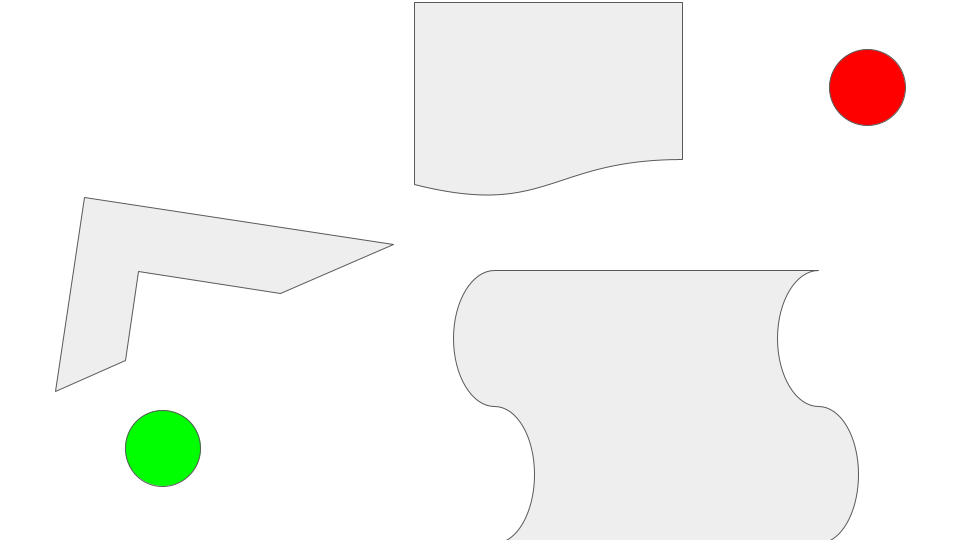
\includegraphics[width=\textwidth]{./assets/rrt_slides/rrt_slides_2.png}}\only<2>{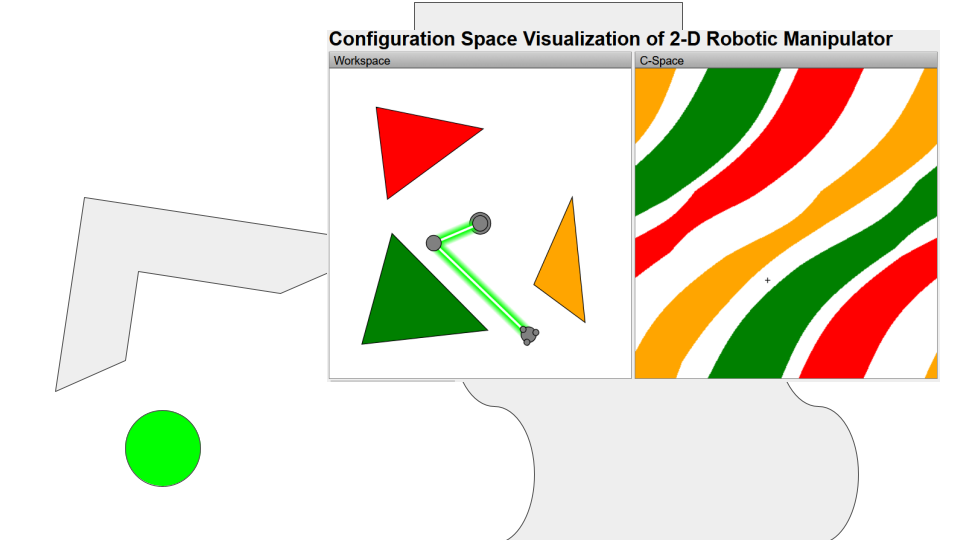
\includegraphics[width=\textwidth]{./assets/rrt_slides/rrt_slides_2.5.png}}
\end{frame}

\begin{frame}{Example \textsc{sbmp} Execution: Sampling}
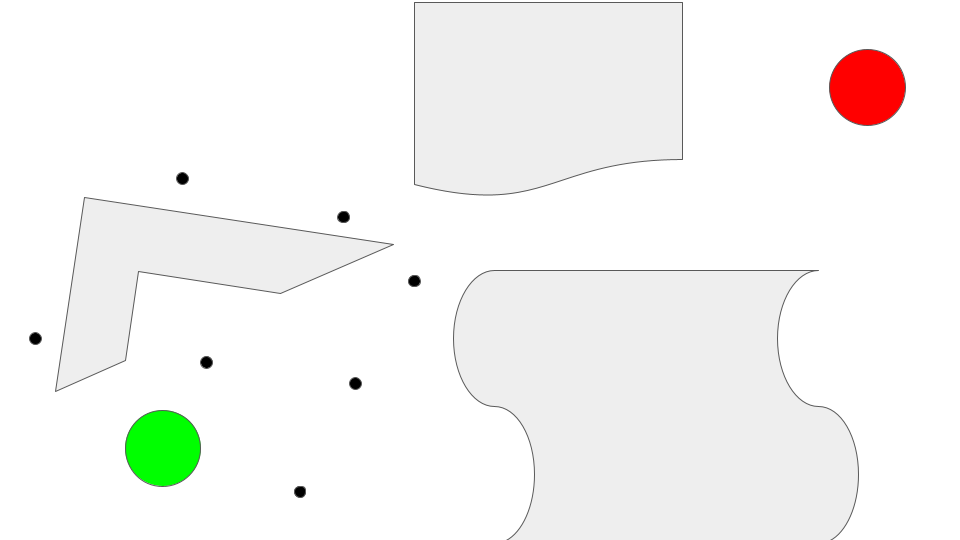
\includegraphics[width=\textwidth]{./assets/rrt_slides/rrt_slides_3.png}
\end{frame}

\begin{frame}{Example \textsc{sbmp} Execution: State Validation}
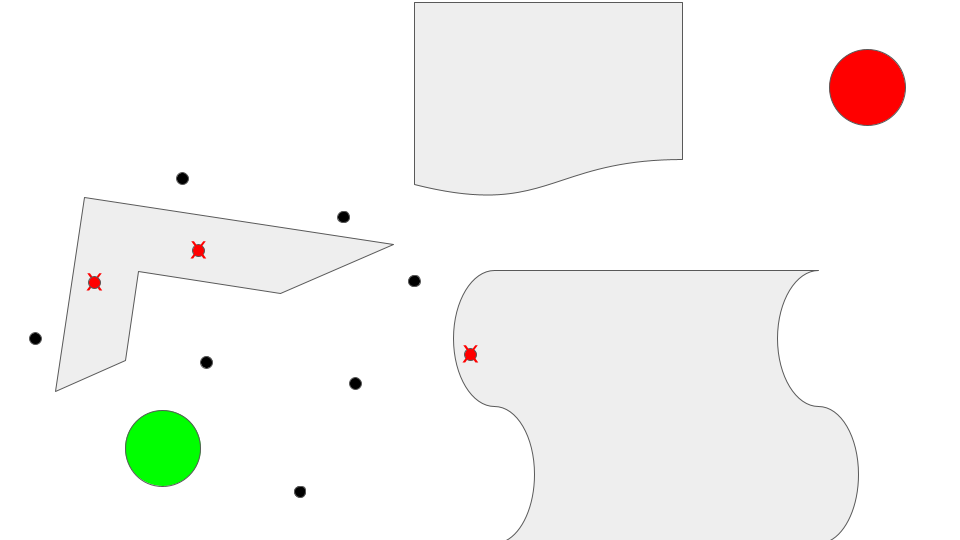
\includegraphics[width=\textwidth]{./assets/rrt_slides/rrt_slides_3.25.png}
\end{frame}

\begin{frame}{Example \textsc{sbmp} Execution: State Validation}
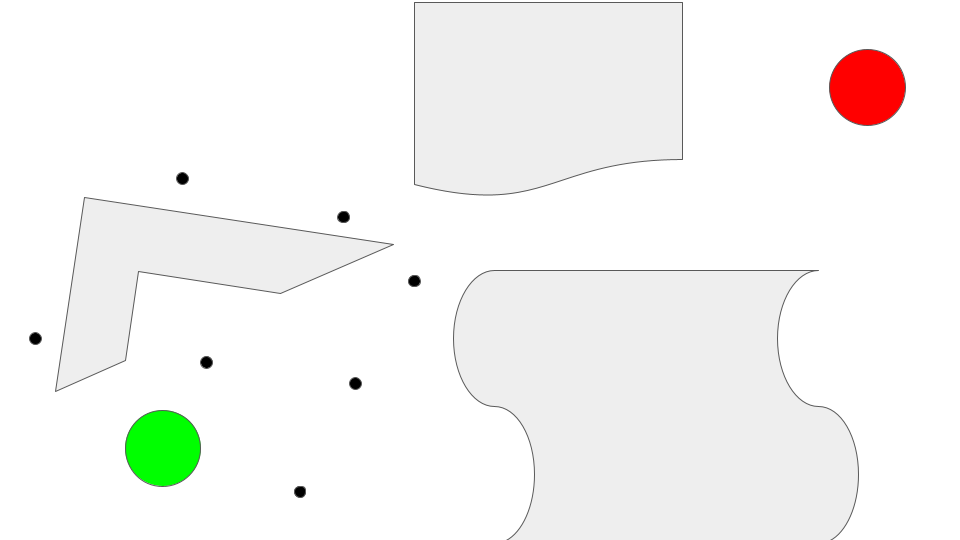
\includegraphics[width=\textwidth]{./assets/rrt_slides/rrt_slides_3.5.png}
\end{frame}

\begin{frame}{Example \textsc{sbmp} Execution: Local Planning}
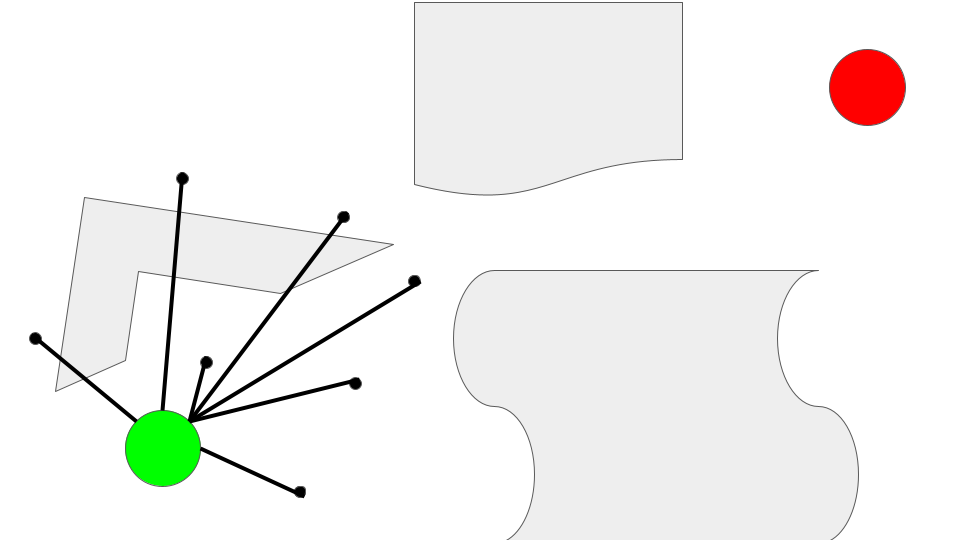
\includegraphics[width=\textwidth]{./assets/rrt_slides/rrt_slides_4.png}
\end{frame}

\begin{frame}{Example \textsc{sbmp} Execution: Collision Checking}
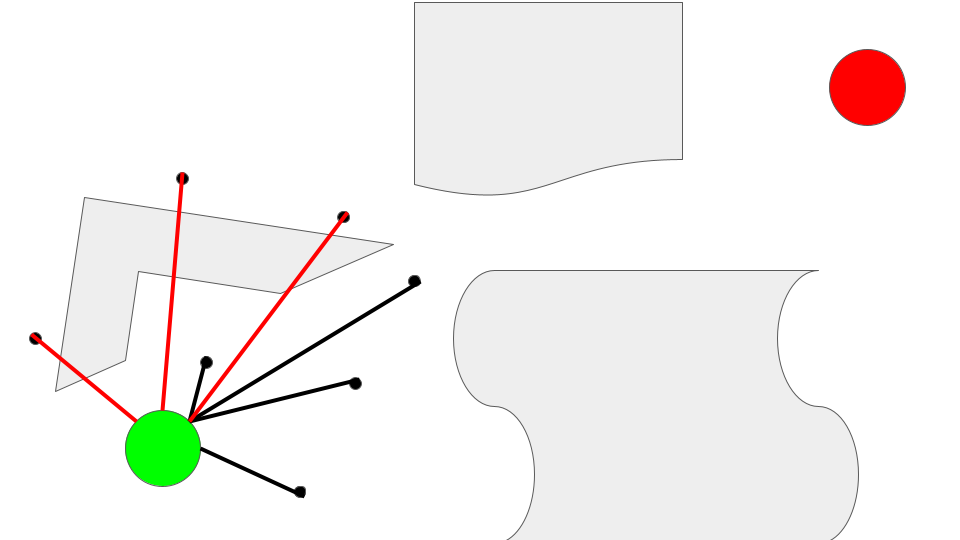
\includegraphics[width=\textwidth]{./assets/rrt_slides/rrt_slides_5.png}
\end{frame}

\begin{frame}{Example \textsc{sbmp} Execution: Motion Validation}
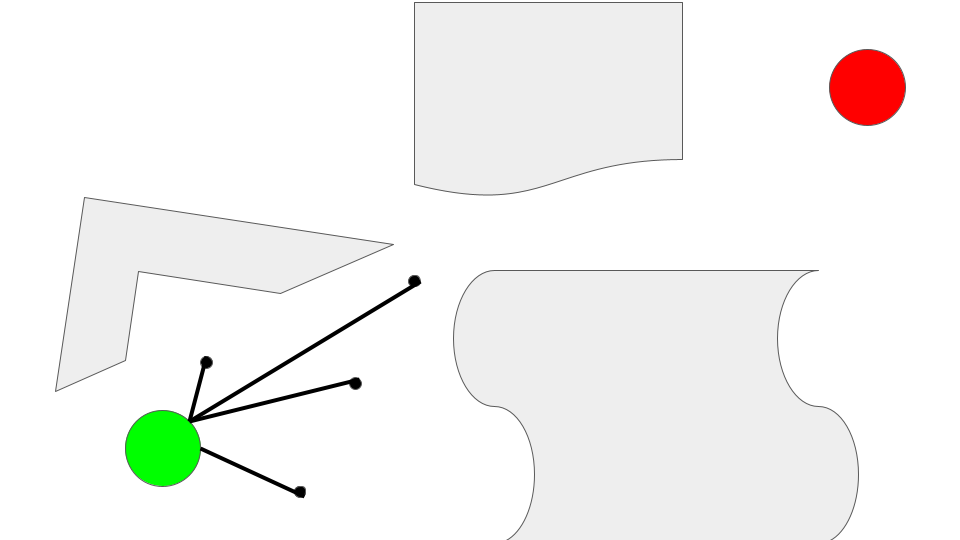
\includegraphics[width=\textwidth]{./assets/rrt_slides/rrt_slides_6.png}
\end{frame}

\begin{frame}{Example \textsc{sbmp} Execution: Generate Whole Graph}
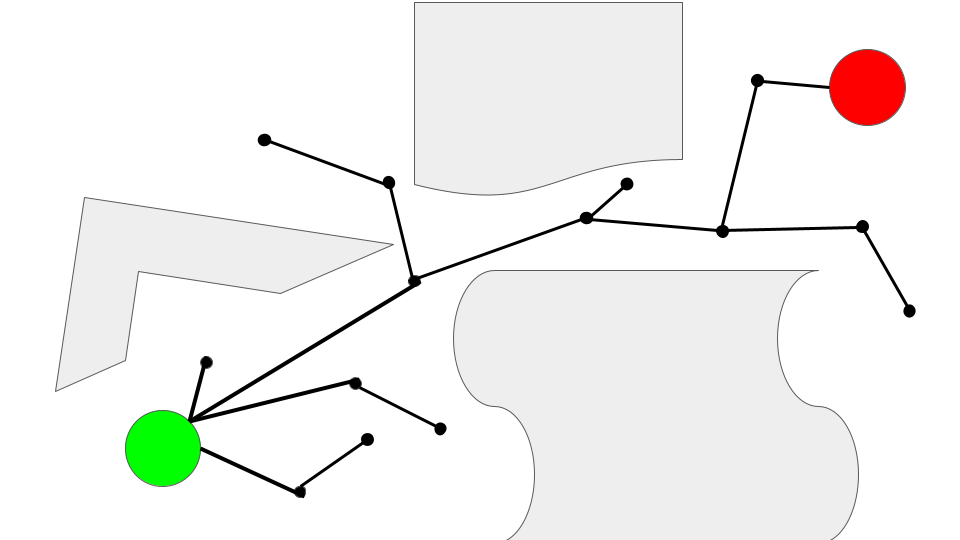
\includegraphics[width=\textwidth]{./assets/rrt_slides/rrt_slides_7.png}
\end{frame}

\begin{frame}{Example \textsc{sbmp} Execution: Find Path}
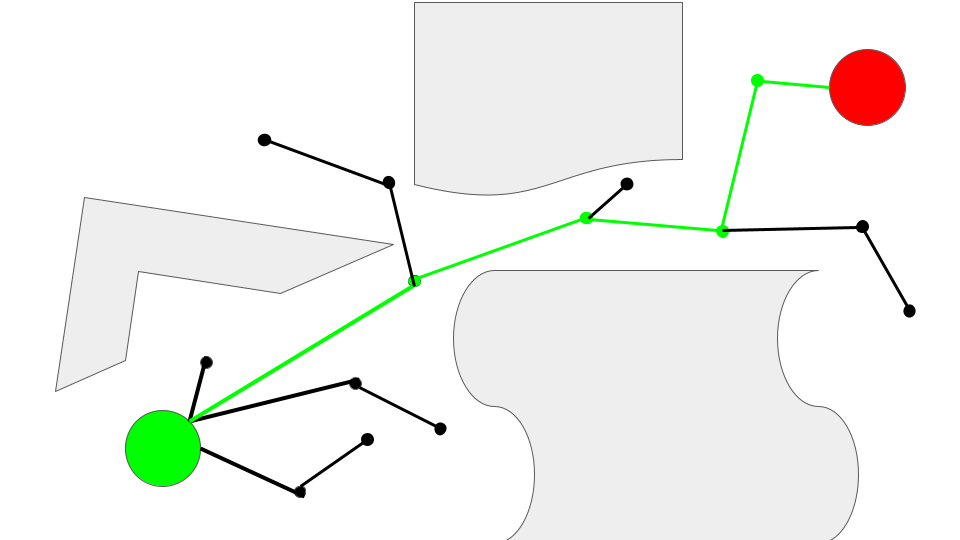
\includegraphics[width=\textwidth]{./assets/rrt_slides/rrt_slides_8.png}
\end{frame}

\subsection{Planning Primitives}

\begin{frame}[label=p_primitives]{Planning Primitives}
% Having gone over the shape of RRT, let's identify what common primitives happen across many sampling-based motion planners.
\pause
\begin{block}{Nearest Neighbors Search (\textsc{nn})}
Part of the sampling function for the configuration space.
\end{block}

\begin{block}{Forward Kinematics (\textsc{fk})}
Maps configuration-space elements to physical space.
\end{block}

\begin{block}{Collision Checking (\textsc{cc})}
Ensures that obstacles do not collide with the robot. Uses many passes of \textsc{fk} in computation. 
\end{block}

\textsc{cc} is conventionally thought of as the most computationally intensive step of the motion planning process. \cite{paper:rrt90}%, so much of the discussion is in optimizing \textsc{cc} and \textsc{fk}

\end{frame}

\begin{frame}
\centering
\textbf{How do we optimize these computationally intensive tasks?}
\end{frame}

\subsection{State of the Art}

\begin{frame}{State of the Art}
\begin{itemize}
\item Motion planning parallelism is typically acheived by running several independent planners in parallel. %What the authors refer to as coarse-grained parallelism
\item Hardware acceleration of motion planning has been explored, but necessarily introduces latency when communicating with the CPU.
\item \textsc{fk} computations are difficult to parallelize due to the robot geometry introducing data dependencies.
\item In order to minimize the total number of \textsc{cc} calls, it is often performed in two steps, \textit{broadphase} and \textit{narrowphase}. \cite{paper:eemp} developed a method for using local sparsity patterns in a parallel manner.
\end{itemize}
\end{frame}

\section{Motions in Microseconds}

\subsection{\textsc{vamp}}

%\cite{paper:MiM} presents Vector-Accelerated Motion Planning (\textsc{vamp}).

%\begin{frame}{Vectorizing Motion Planning}
%\pause
%\begin{block}{Vector}
%A \textit{vector} is a fixed-length sequence of scalar values.
%\end{block}
%
%\begin{block}{Vectorized Operation}
%A \textit{vectorized operation} acts on all values within the vector. This operation must be done independently, in parallel.
%\end{block}
%
%\pause
%\cite{paper:MiM} chose to focus on CPU-level parallelism, rather than GPU-level, process-level, or thread-level parallelism, so as to incur less overhead.
%\end{frame}

\begin{frame}{Vector Accelerated Motion Planning (\textsc{vamp})}
\textsc{vamp} presents a novel planner that uses \textit{fine-grained} instruction-level parallelism to achieve substantial speedups.

\vspace{10px}

\pause
\textsc{vamp}'s innovations over State of the Art:
\begin{itemize}
\item 1. Struct-of-Arrays data representation
\item 2. Raked Motion Validator implementation
\item 3. Geometric Intersection Tests
\item 4. Tracing Compiler
\end{itemize}
\end{frame}

\begin{frame}{Struct-of-Arrays}
%The more intuitive data representation is AoS, but
\centering
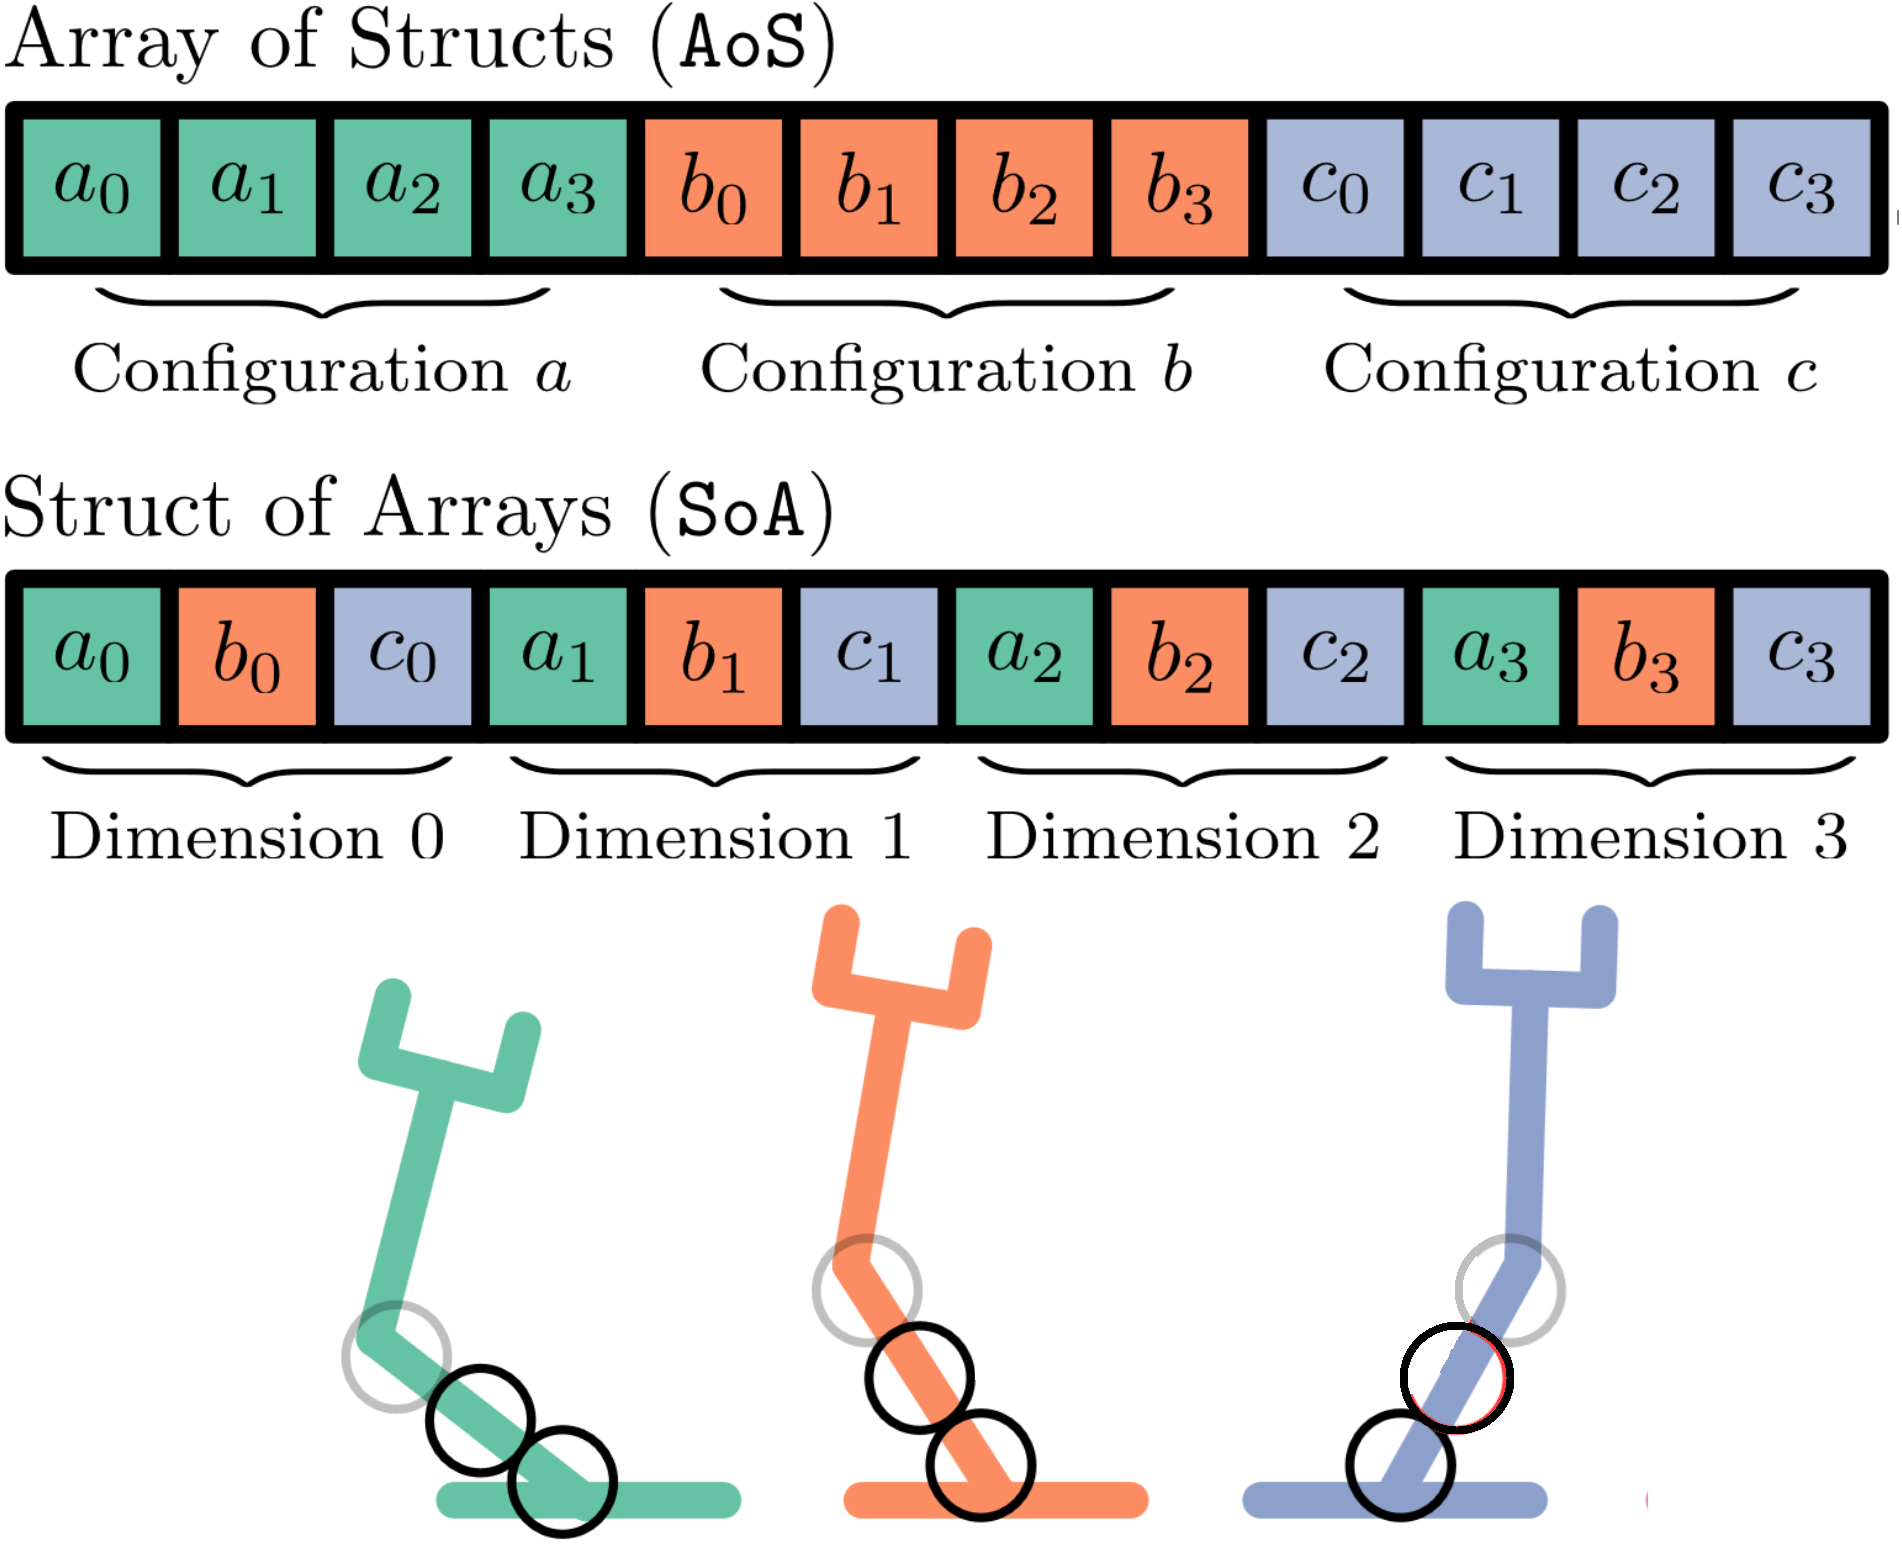
\includegraphics[height=0.8\textheight]{./assets/soa_aos_bar.png}
\end{frame}


\begin{frame}{Raked Motion Validator}
\centering
\only<1>{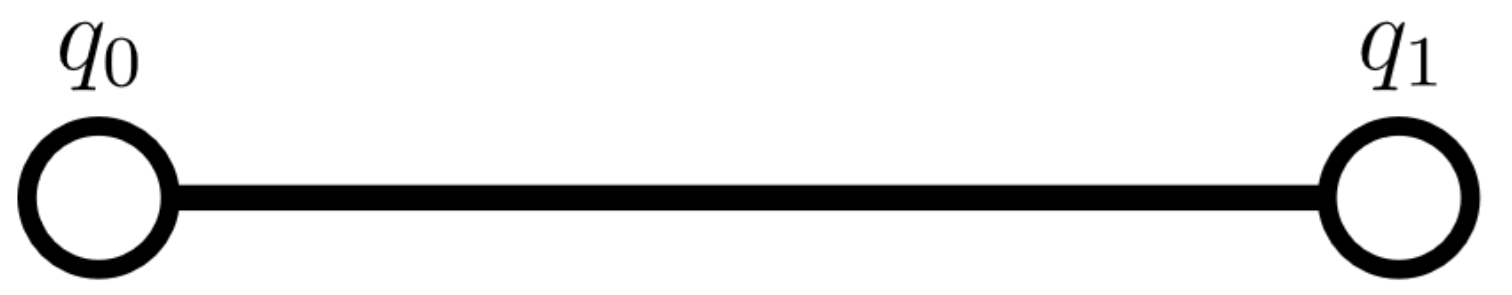
\includegraphics[width=\textwidth]{./assets/rake/rake_1.png}
}\only<2>{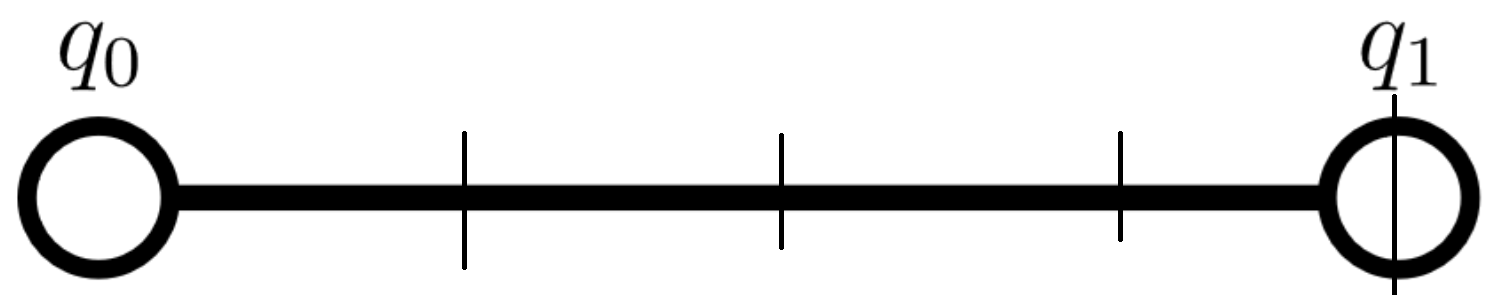
\includegraphics[width=\textwidth]{./assets/rake/rake_1_lines.png}
}\only<3>{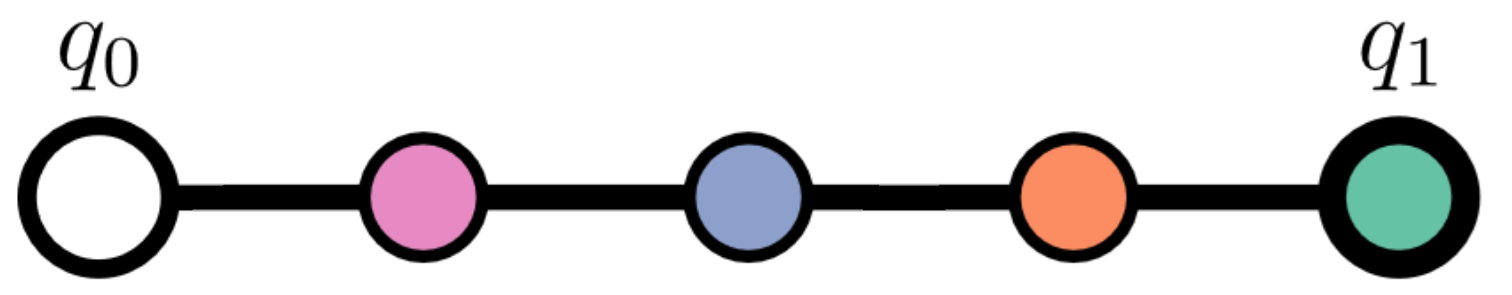
\includegraphics[width=\textwidth]{./assets/rake/rake_2.png}
}\only<4>{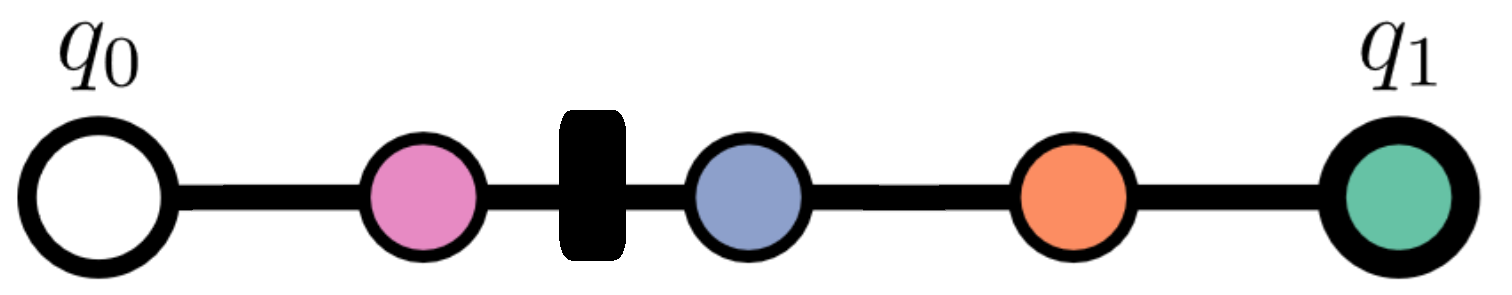
\includegraphics[width=\textwidth]{./assets/rake/rake_2_obst.png}
}\only<5>{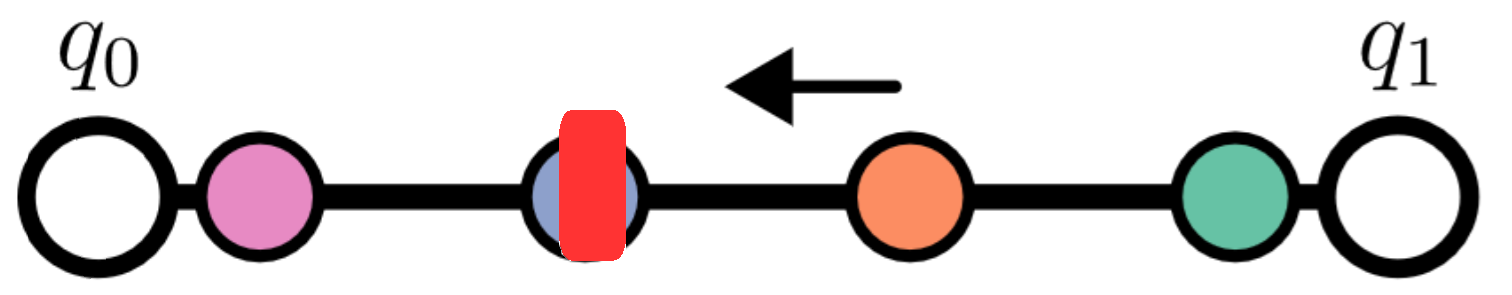
\includegraphics[width=\textwidth]{./assets/rake/rake_3_obst.png}
}\only<1>{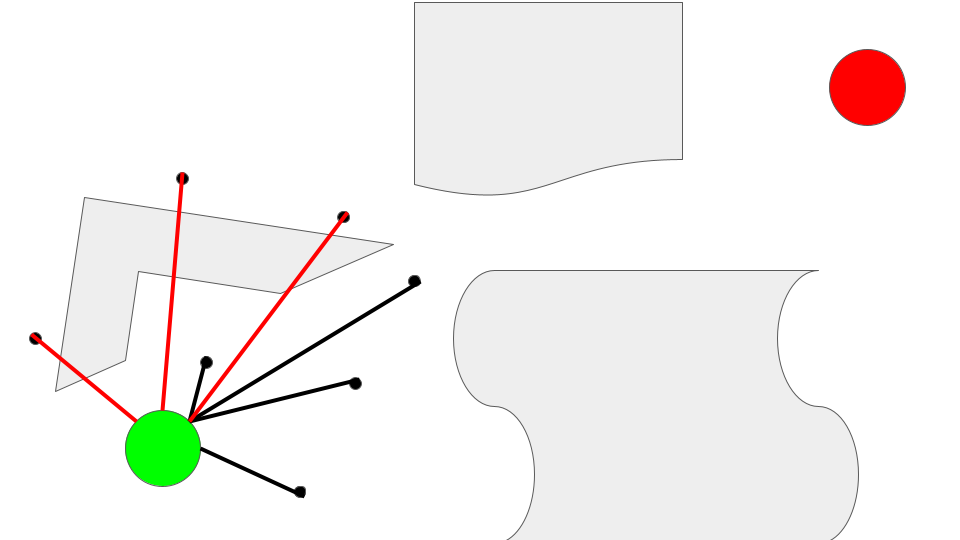
\includegraphics[width=0.6\textwidth]{./assets/rrt_slides/rrt_slides_5.png}
}\only<2>{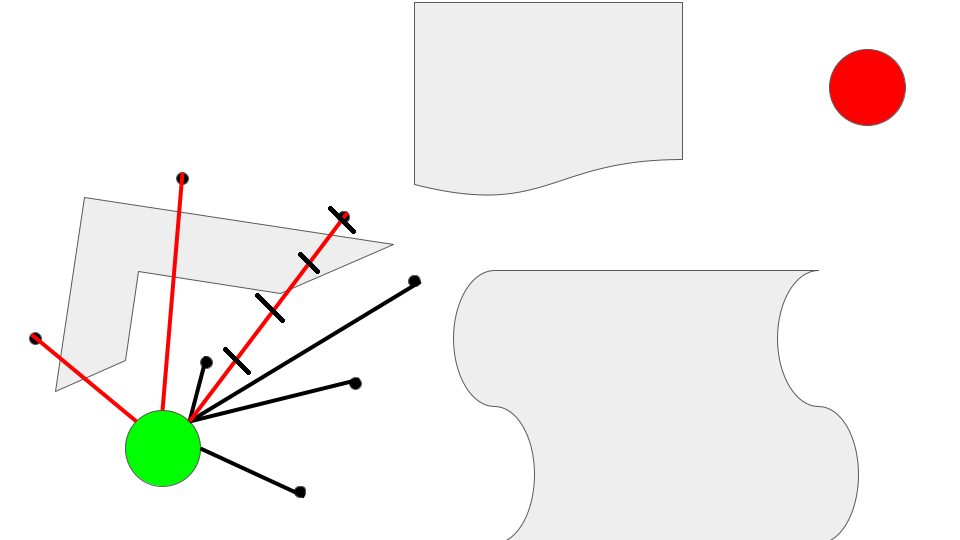
\includegraphics[width=0.6\textwidth]{./assets/rake/rrt_slides_5.png}
}\only<3>{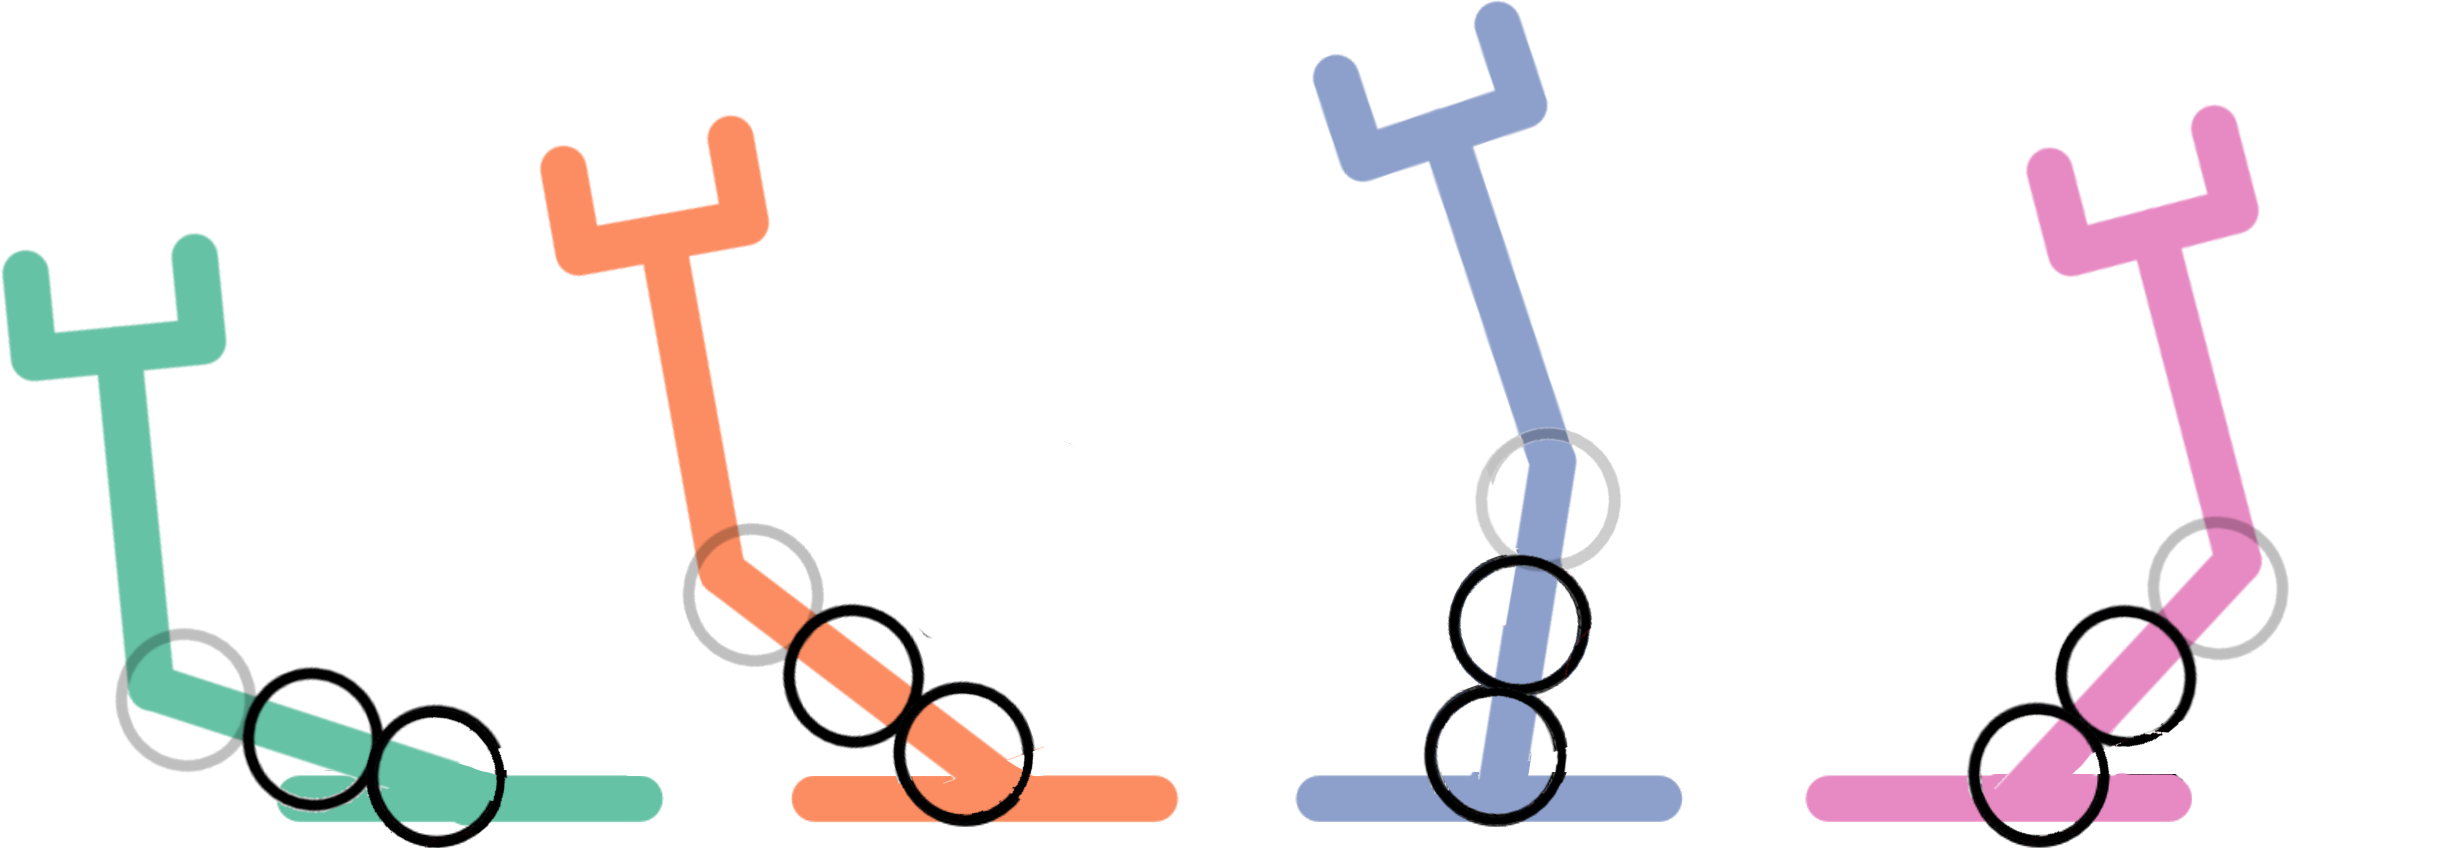
\includegraphics[width=\textwidth]{./assets/rake/arm_no_obsts.png}
}\only<4>{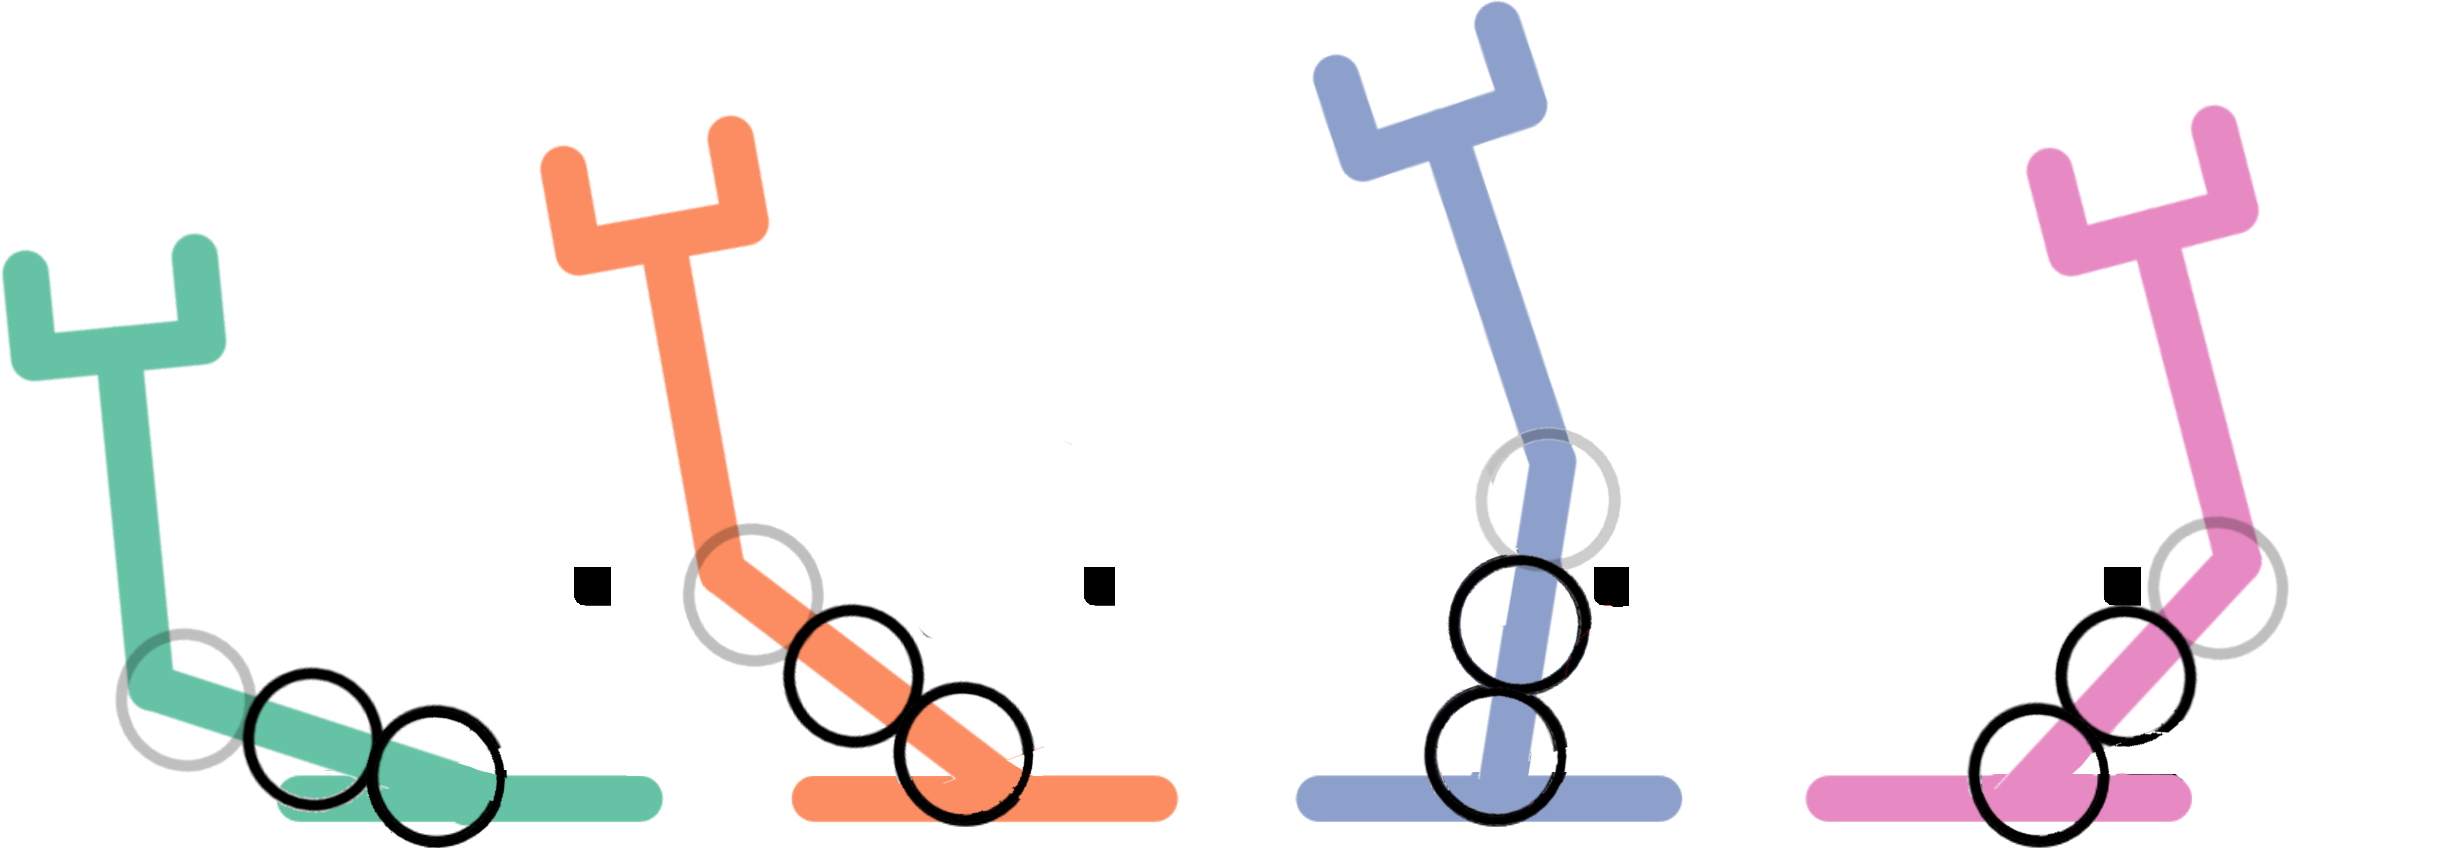
\includegraphics[width=\textwidth]{./assets/rake/arm_no_int.png}
}\only<5>{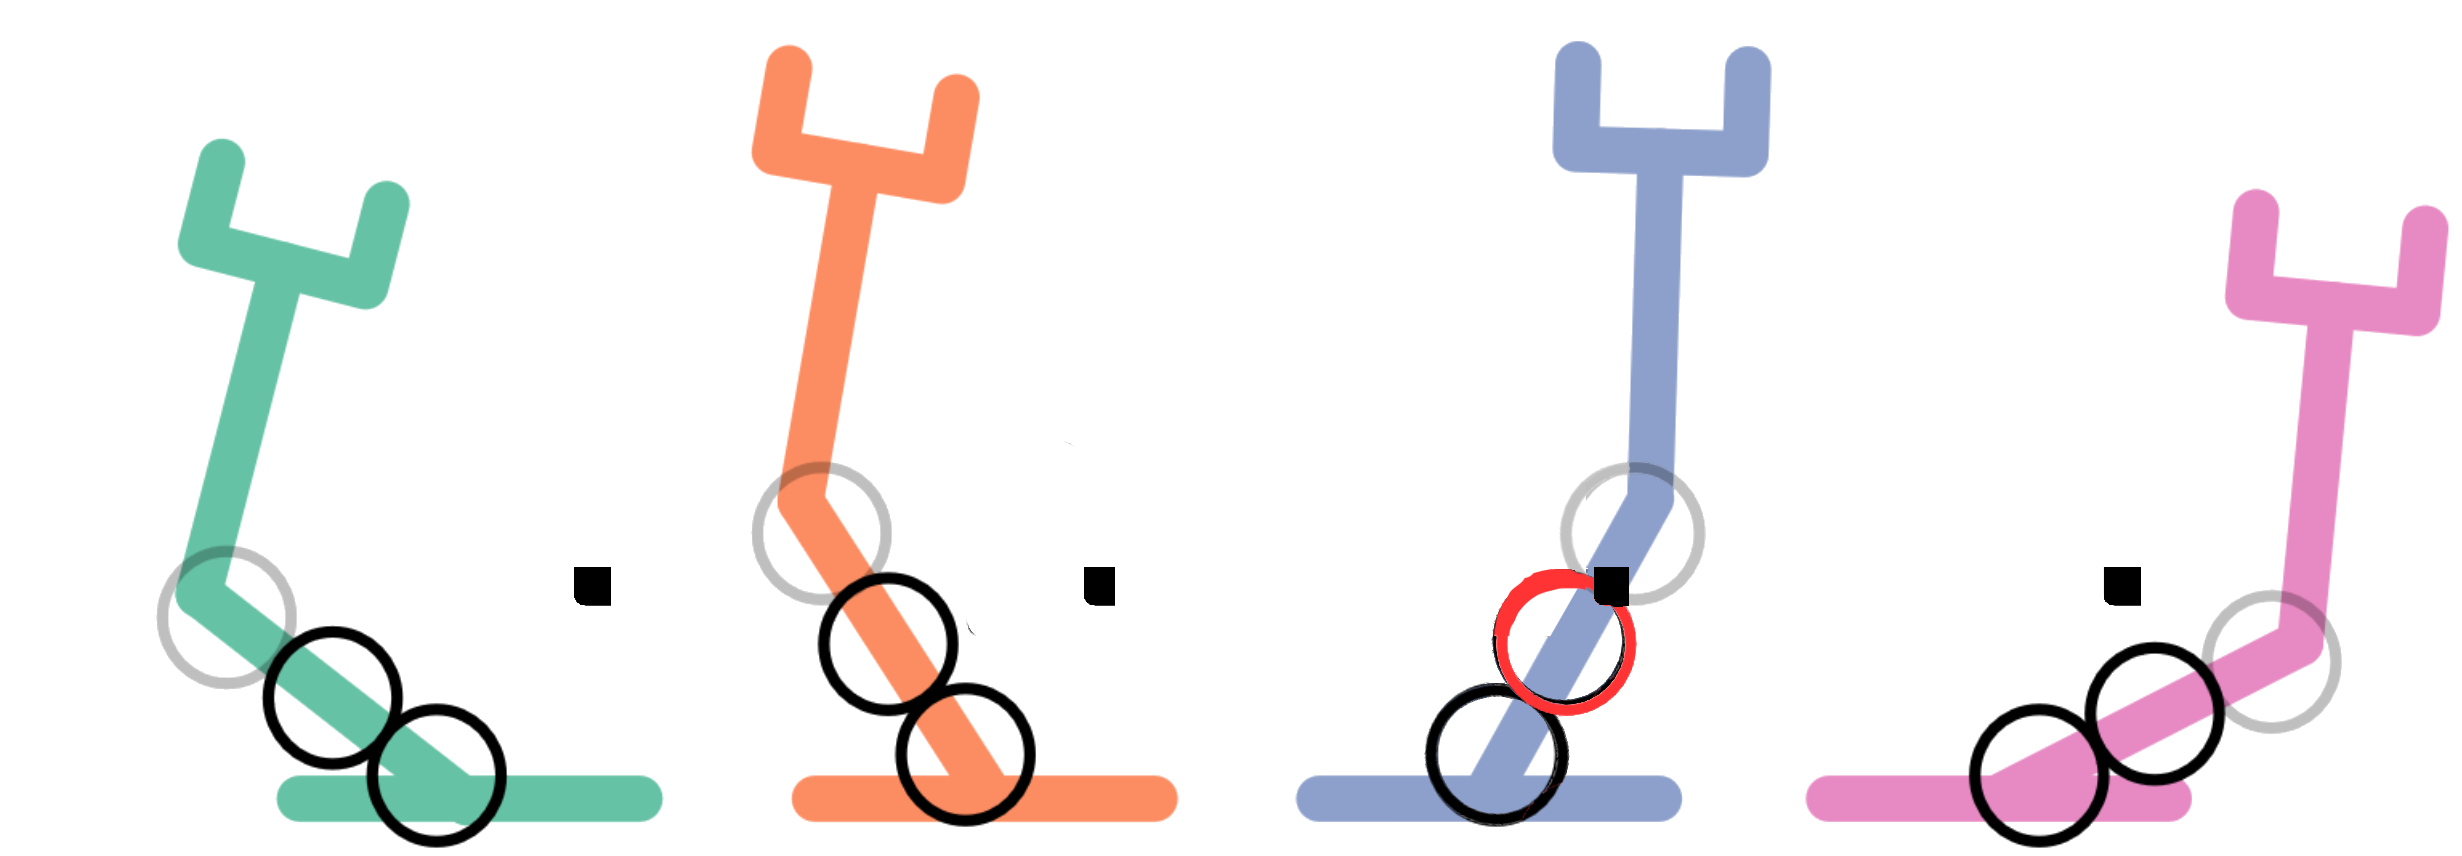
\includegraphics[width=\textwidth]{./assets/rake/arm_int.png}
}%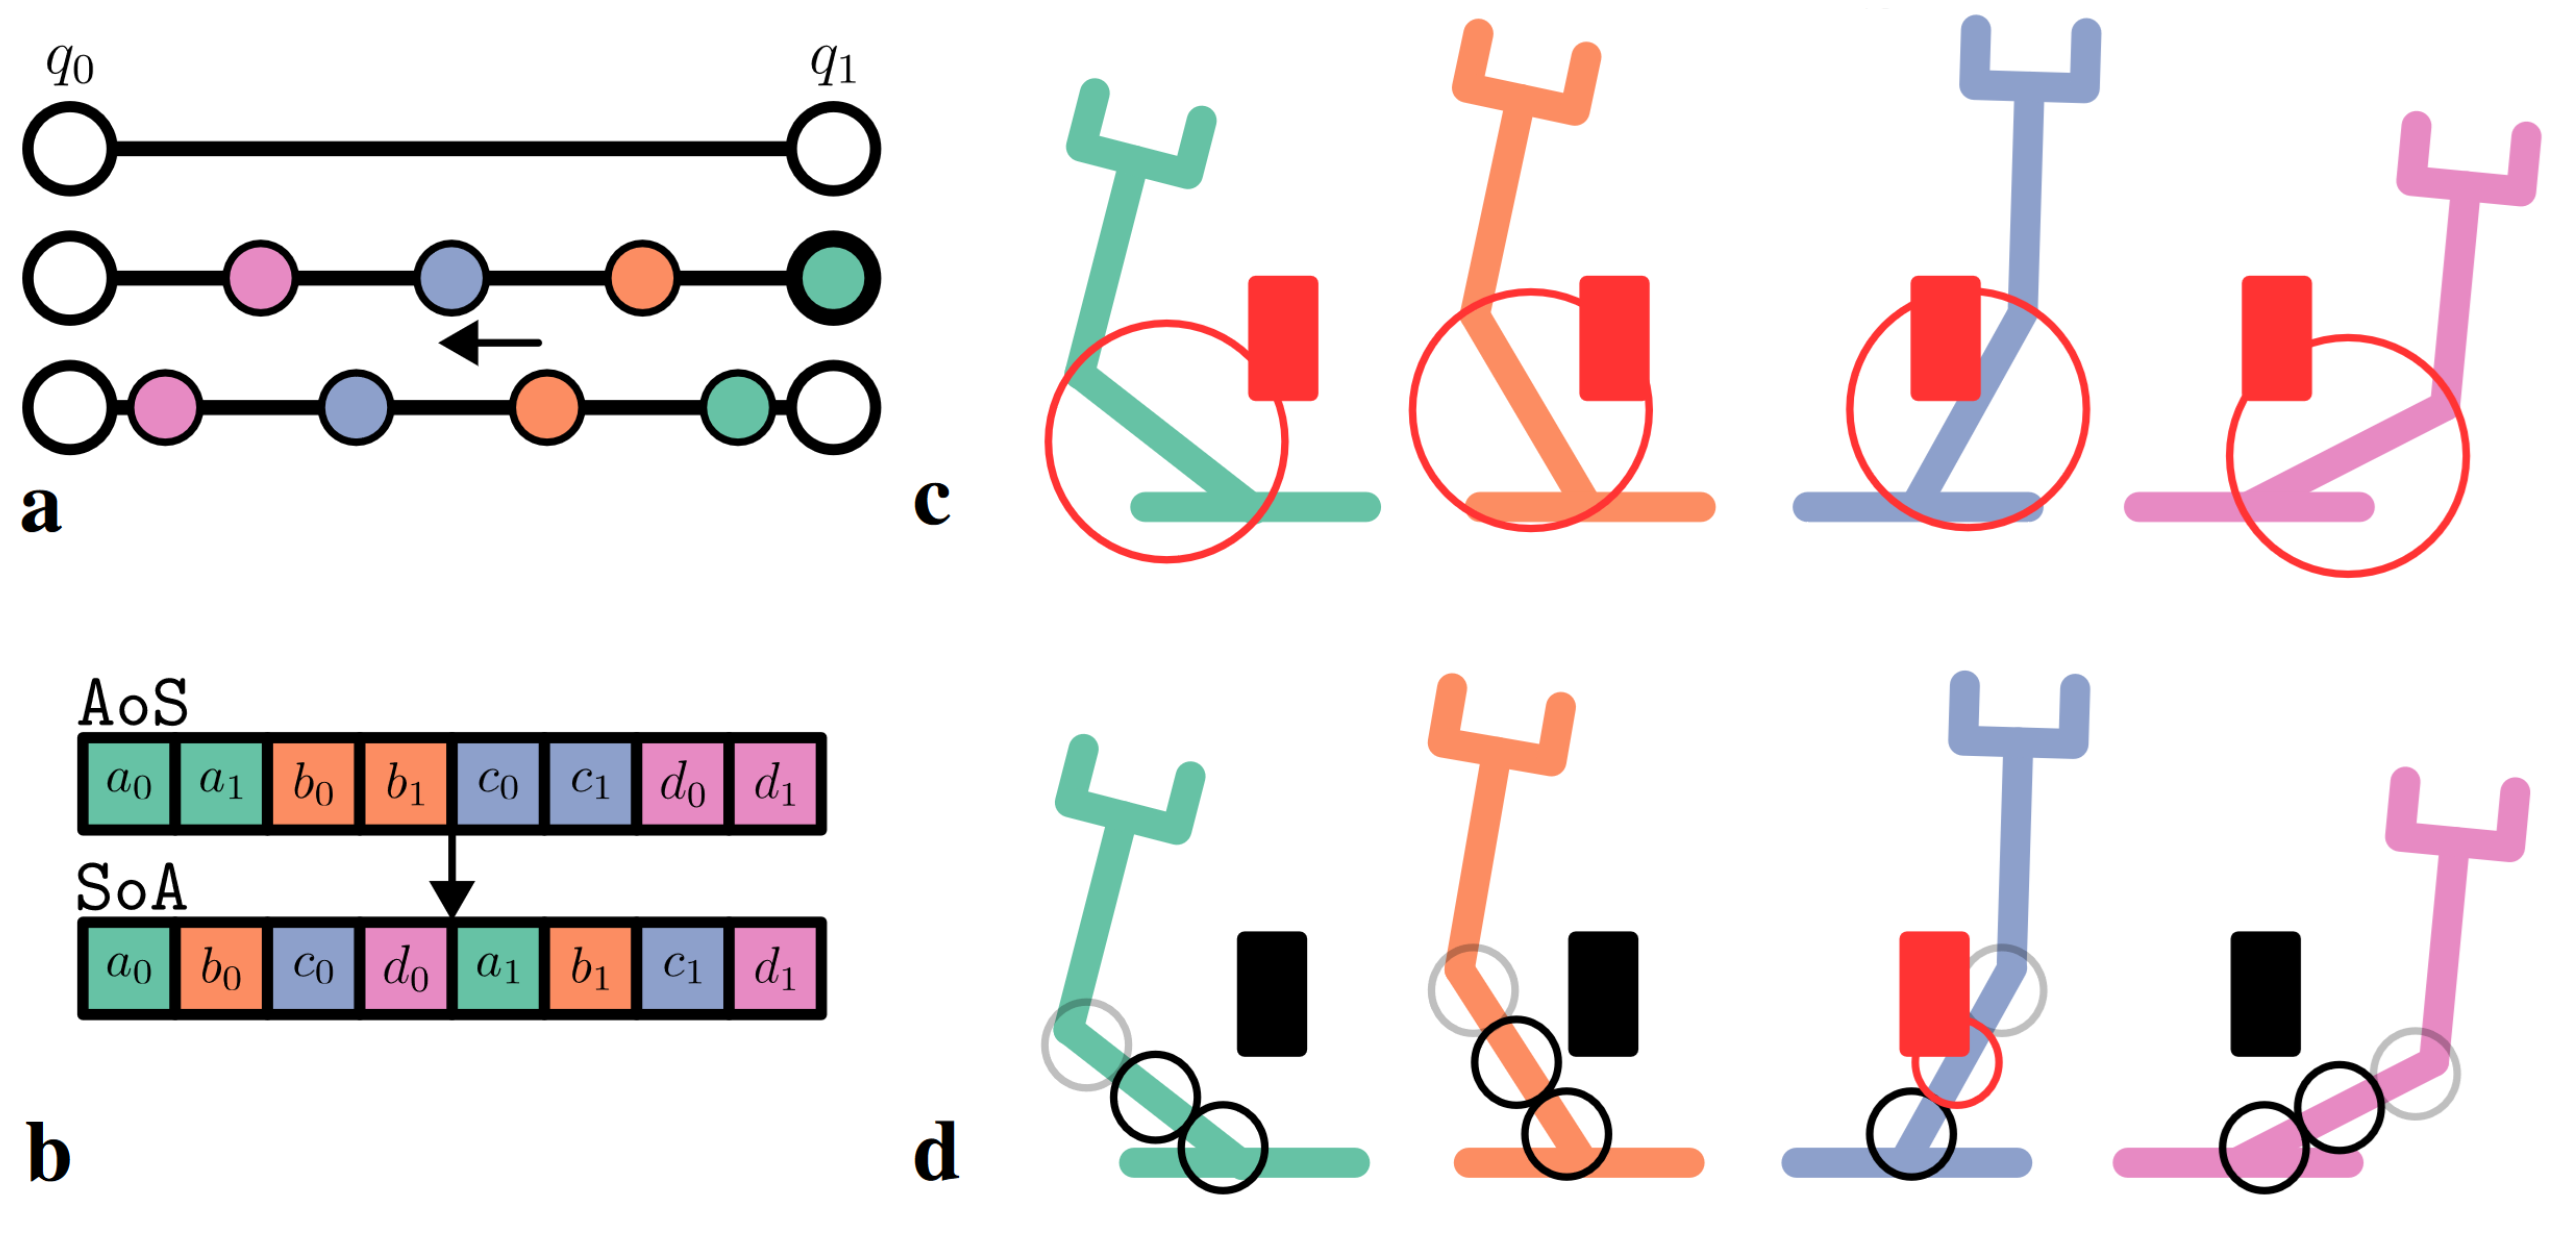
\includegraphics[width=\textwidth]{./assets/mim_raked_mv_rearrange.png}
\end{frame}

\begin{frame}{Geometric Intersection Tests}
\begin{columns}
\begin{column}{0.5\textwidth}
By representing the robot as a system of geometric objects, intersection tests between pairs of objects can be vectorized.

\vspace{10px}

This approach does away with the staged broadphase and narrowphase approach to collision checking, but focuses soley on narrowphase.
\end{column}
\begin{column}{0.5\textwidth}
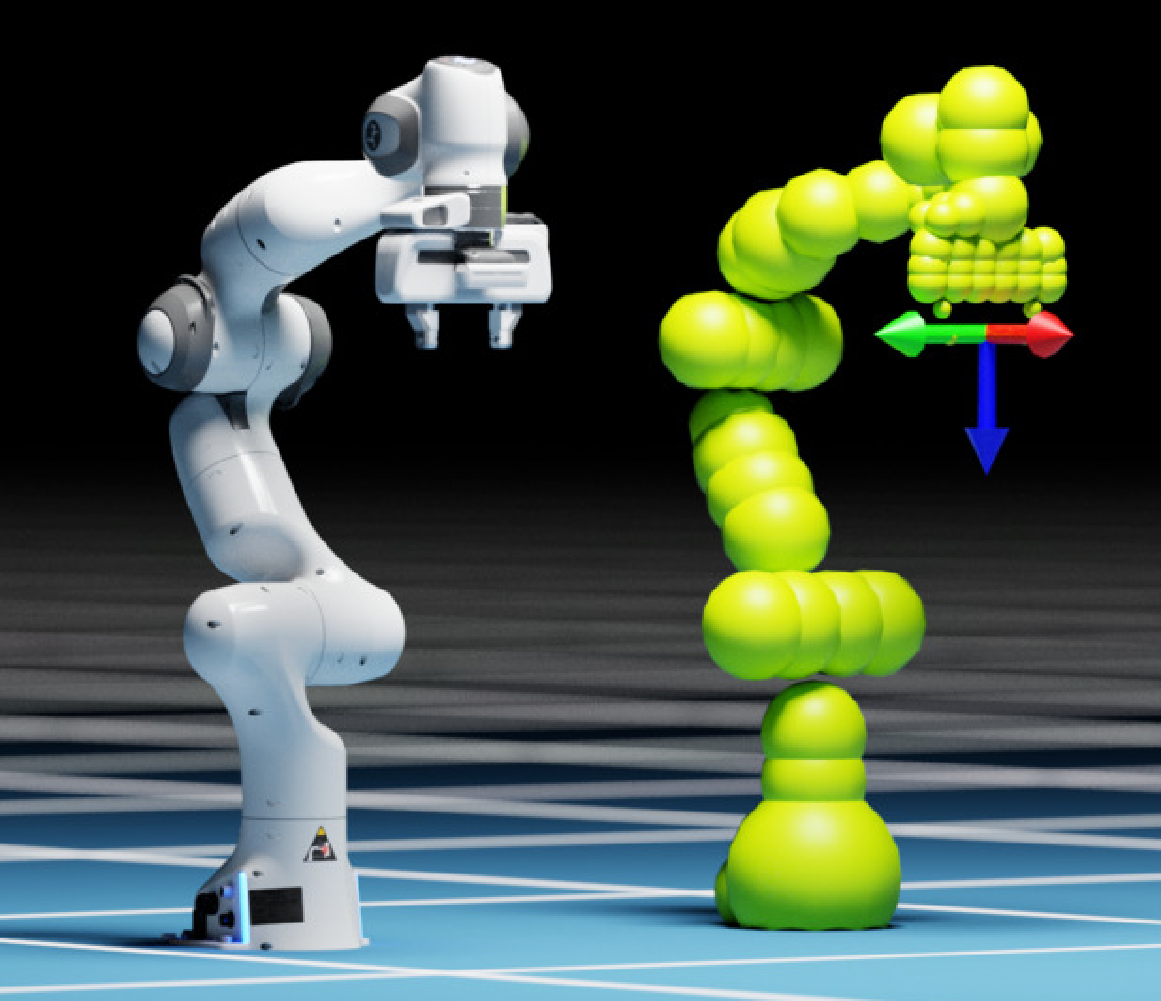
\includegraphics[width=\textwidth]{./assets/panda_spheres.png}
\end{column}
\end{columns}
\end{frame}

\begin{frame}{Tracing Compiler}
%\textsc{fk} has been difficult to parallelize with prior approaches due to data dependencies between link transforms in the kinematic chain.
To vectorize \textsc{fk}:
\begin{itemize}
\item Trace the operations of the robot's kinematics from a \textsc{urdf} file.
\item Generate a vector configuration structure for a batch of configurations. 
\item Output a minimal set of operations to compute the traced function as an unrolled loop.
\end{itemize}

Notably, this tracing technique generates optimized \textsc{fk} implementations at compile time through automatic code generation.
\end{frame}

\section{Strengths \& Weaknesses}

\subsection{Strengths}

\begin{frame}{Strengths}
\begin{columns}
\begin{column}{0.5\textwidth}
With straightforward architechtural optimizations, the authors get upwards of 500$\times$ speedups over PyBullet, and 100-200$\times$ over MoveIt, both using \textsc{ompl} for the motion planning implementation.
\end{column}
\begin{column}{0.5\textwidth}
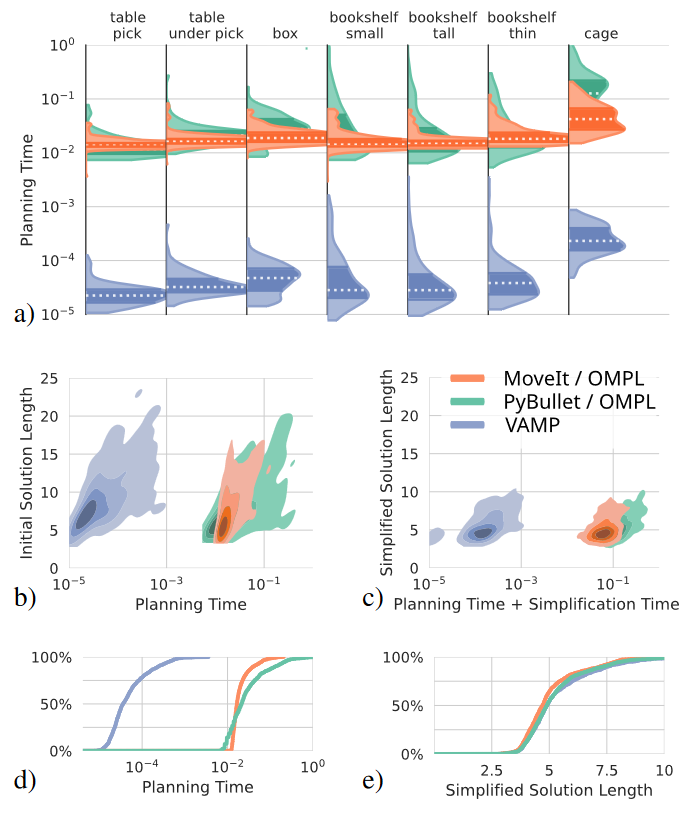
\includegraphics[width=\textwidth]{./assets/panda_graphs.png}
\end{column}
\end{columns}

%The authors made innovations that no one before them realized would matter so significantly.
\end{frame}

\subsection{Weaknesses}

\begin{frame}{Weaknesses}
The authors don't show an ablation study of which optimizations make which end-to-end performance impacts.
\vspace{5px}\pause

The paper does not describe what impacts the optimizations have as the problem size scales. The below table shows massive differences between the 7DOF Panda and the 8DOF Fetch robot.

\begin{table}[width=0.8\textwidth]

\centering
  \sisetup{table-format = {$\times$ 4.2}, table-align-text-before = false}
  \begin{tabular}{ll*{5}{@{\hspace{4pt}} >{$\times$} S}}
  \toprule
        & vs \textsc{vamp} & \multicolumn{1}{c}{Mean} & \multicolumn{1}{c}{Q1} & \multicolumn{1}{c}{Median} & \multicolumn{1}{c}{Q3} & \multicolumn{1}{c}{95\%} \\
  \midrule
  Panda & PyBullet & 403.03 & 797.69  & 888.46   & 786.02 & 360.09 \\
        & MoveIt  & 55.36  & 2594.63 & 1126.30  & 247.47 & 28.35  \\
  \midrule
  Fetch & PyBullet & 108.01 & 314.31  & 434.04   & 212.13 & 86.64  \\
        & MoveIt   & 13.39  & 60.95   & 34.47    & 16.51  & 11.86  \\
  \bottomrule
\end{tabular}
\end{table}

\end{frame}

\section{Future Work}

\begin{frame}{Avenues for Future Work}
\begin{itemize}
\item Measure and identify precise bottlenecks within \textsc{sbmp}
\item Optimize geometric intersection tests further
%\item Algorithm-compute codesign
\end{itemize}

\end{frame}

\begin{frame}{Measuring Bottlenecks}
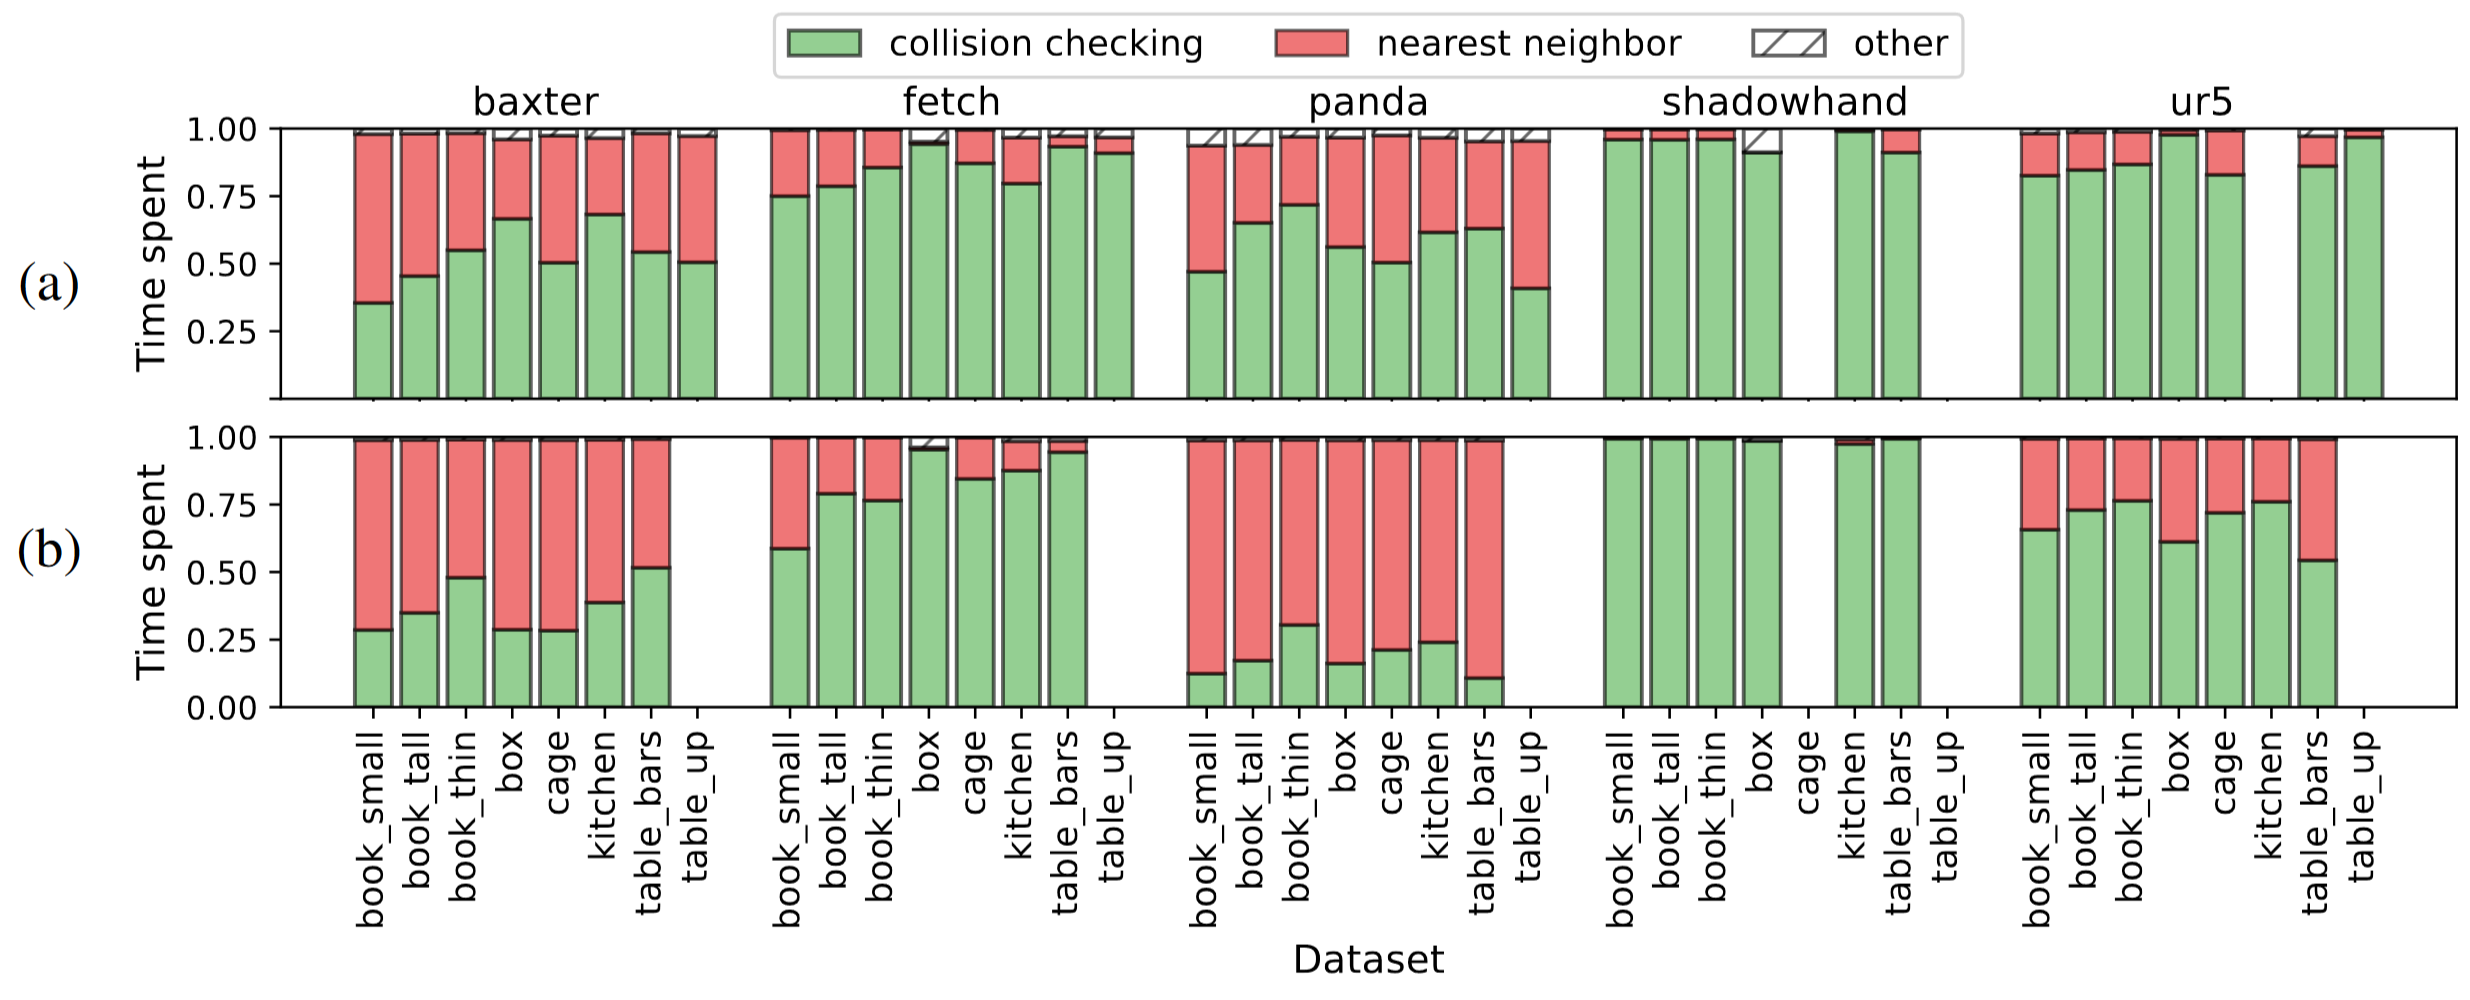
\includegraphics[width=\textwidth]{./assets/cc_nn_zoom.png}
\end{frame}

\begin{frame}{Bounding Volume Fidelity Research}
\begin{itemize}
\item Exploit structured information about manipulator \& environment
\item Explore non-sphere geometric representations of colliders (eg trimeshes, capsules)
\item Explore bounding volume hierarchy fidelity
\end{itemize}
\centering
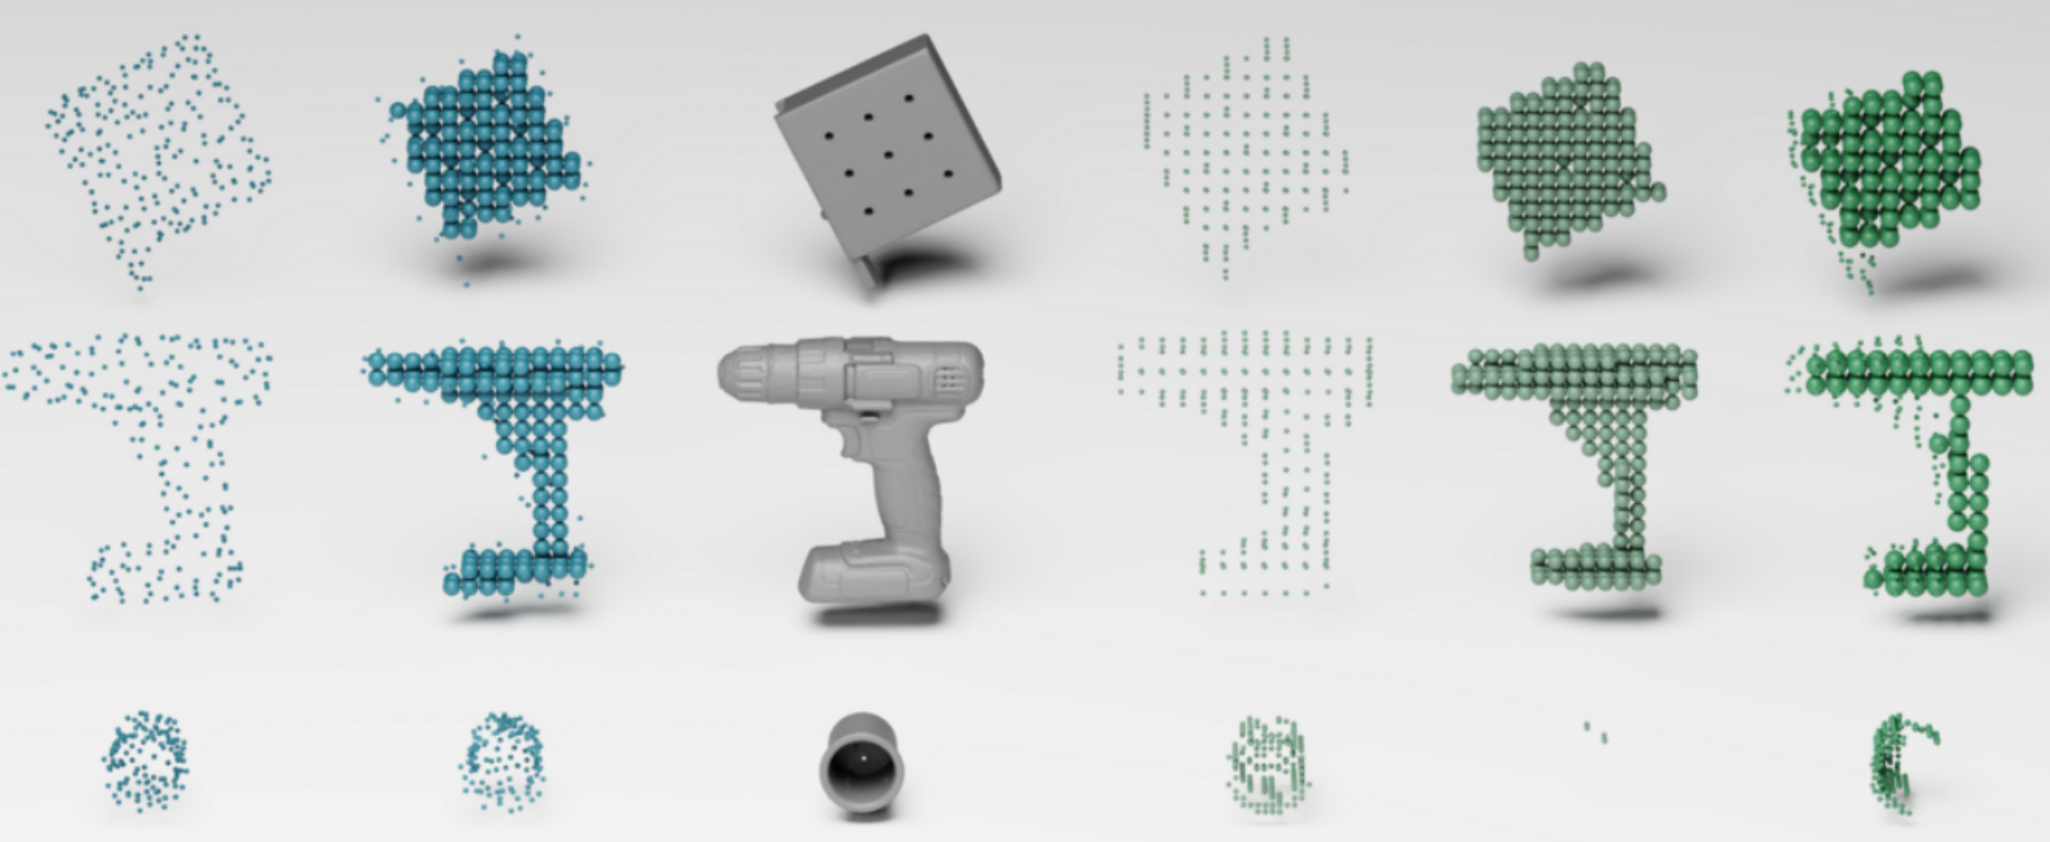
\includegraphics[height=0.37\textheight]{./assets/geom_fidelity.png}
\end{frame}

%\begin{frame}{Algorithm-compute Codesign}
%When should we devote resources to one motion primitive over another? How do we separate \textit{what} we compute from \textit{how}?
%
%\todo{Paraphrase Radhika's description, find picture}
%\end{frame}

\begin{frame}{End of Presentation}
\end{frame}

\section{Extra Figures}

\begin{frame}{Raked Motion Validator Implementation}
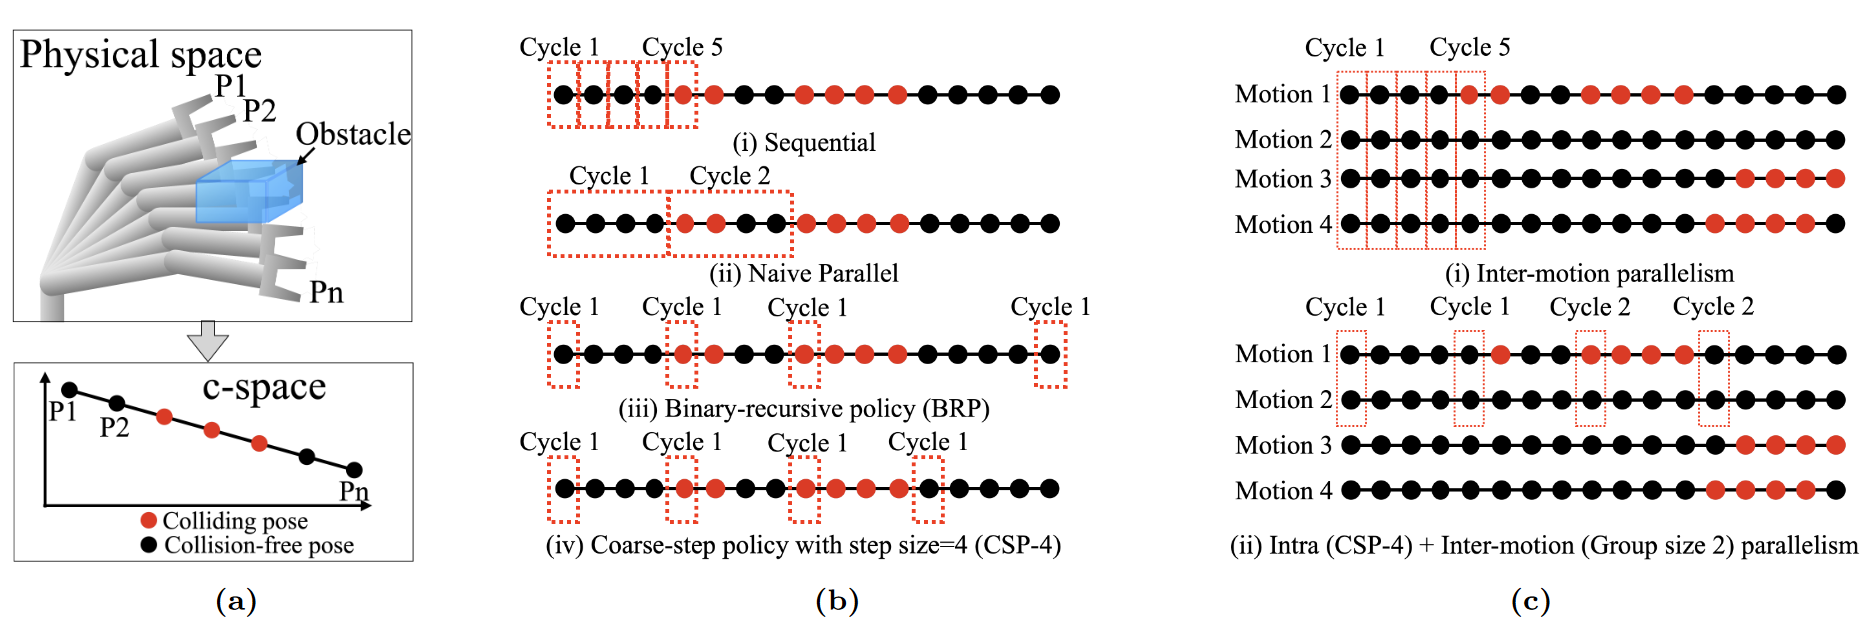
\includegraphics[width=\textwidth]{./assets/eemp_mv.png}

[\cite{paper:eemp}]
\end{frame}

\begin{frame}{2D Configuration Space Visualization}
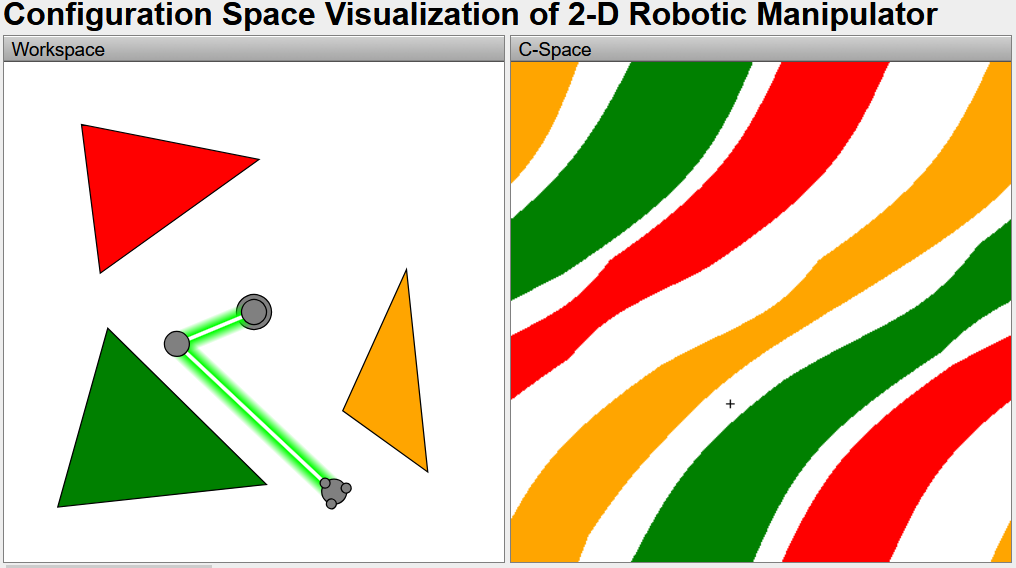
\includegraphics[width=\textwidth]{./assets/c_space.png}
[https://www.cs.unc.edu/~jeffi/c-space/robot.xhtml]
\end{frame}

\begin{frame}{Edge Validation vs State Validation}
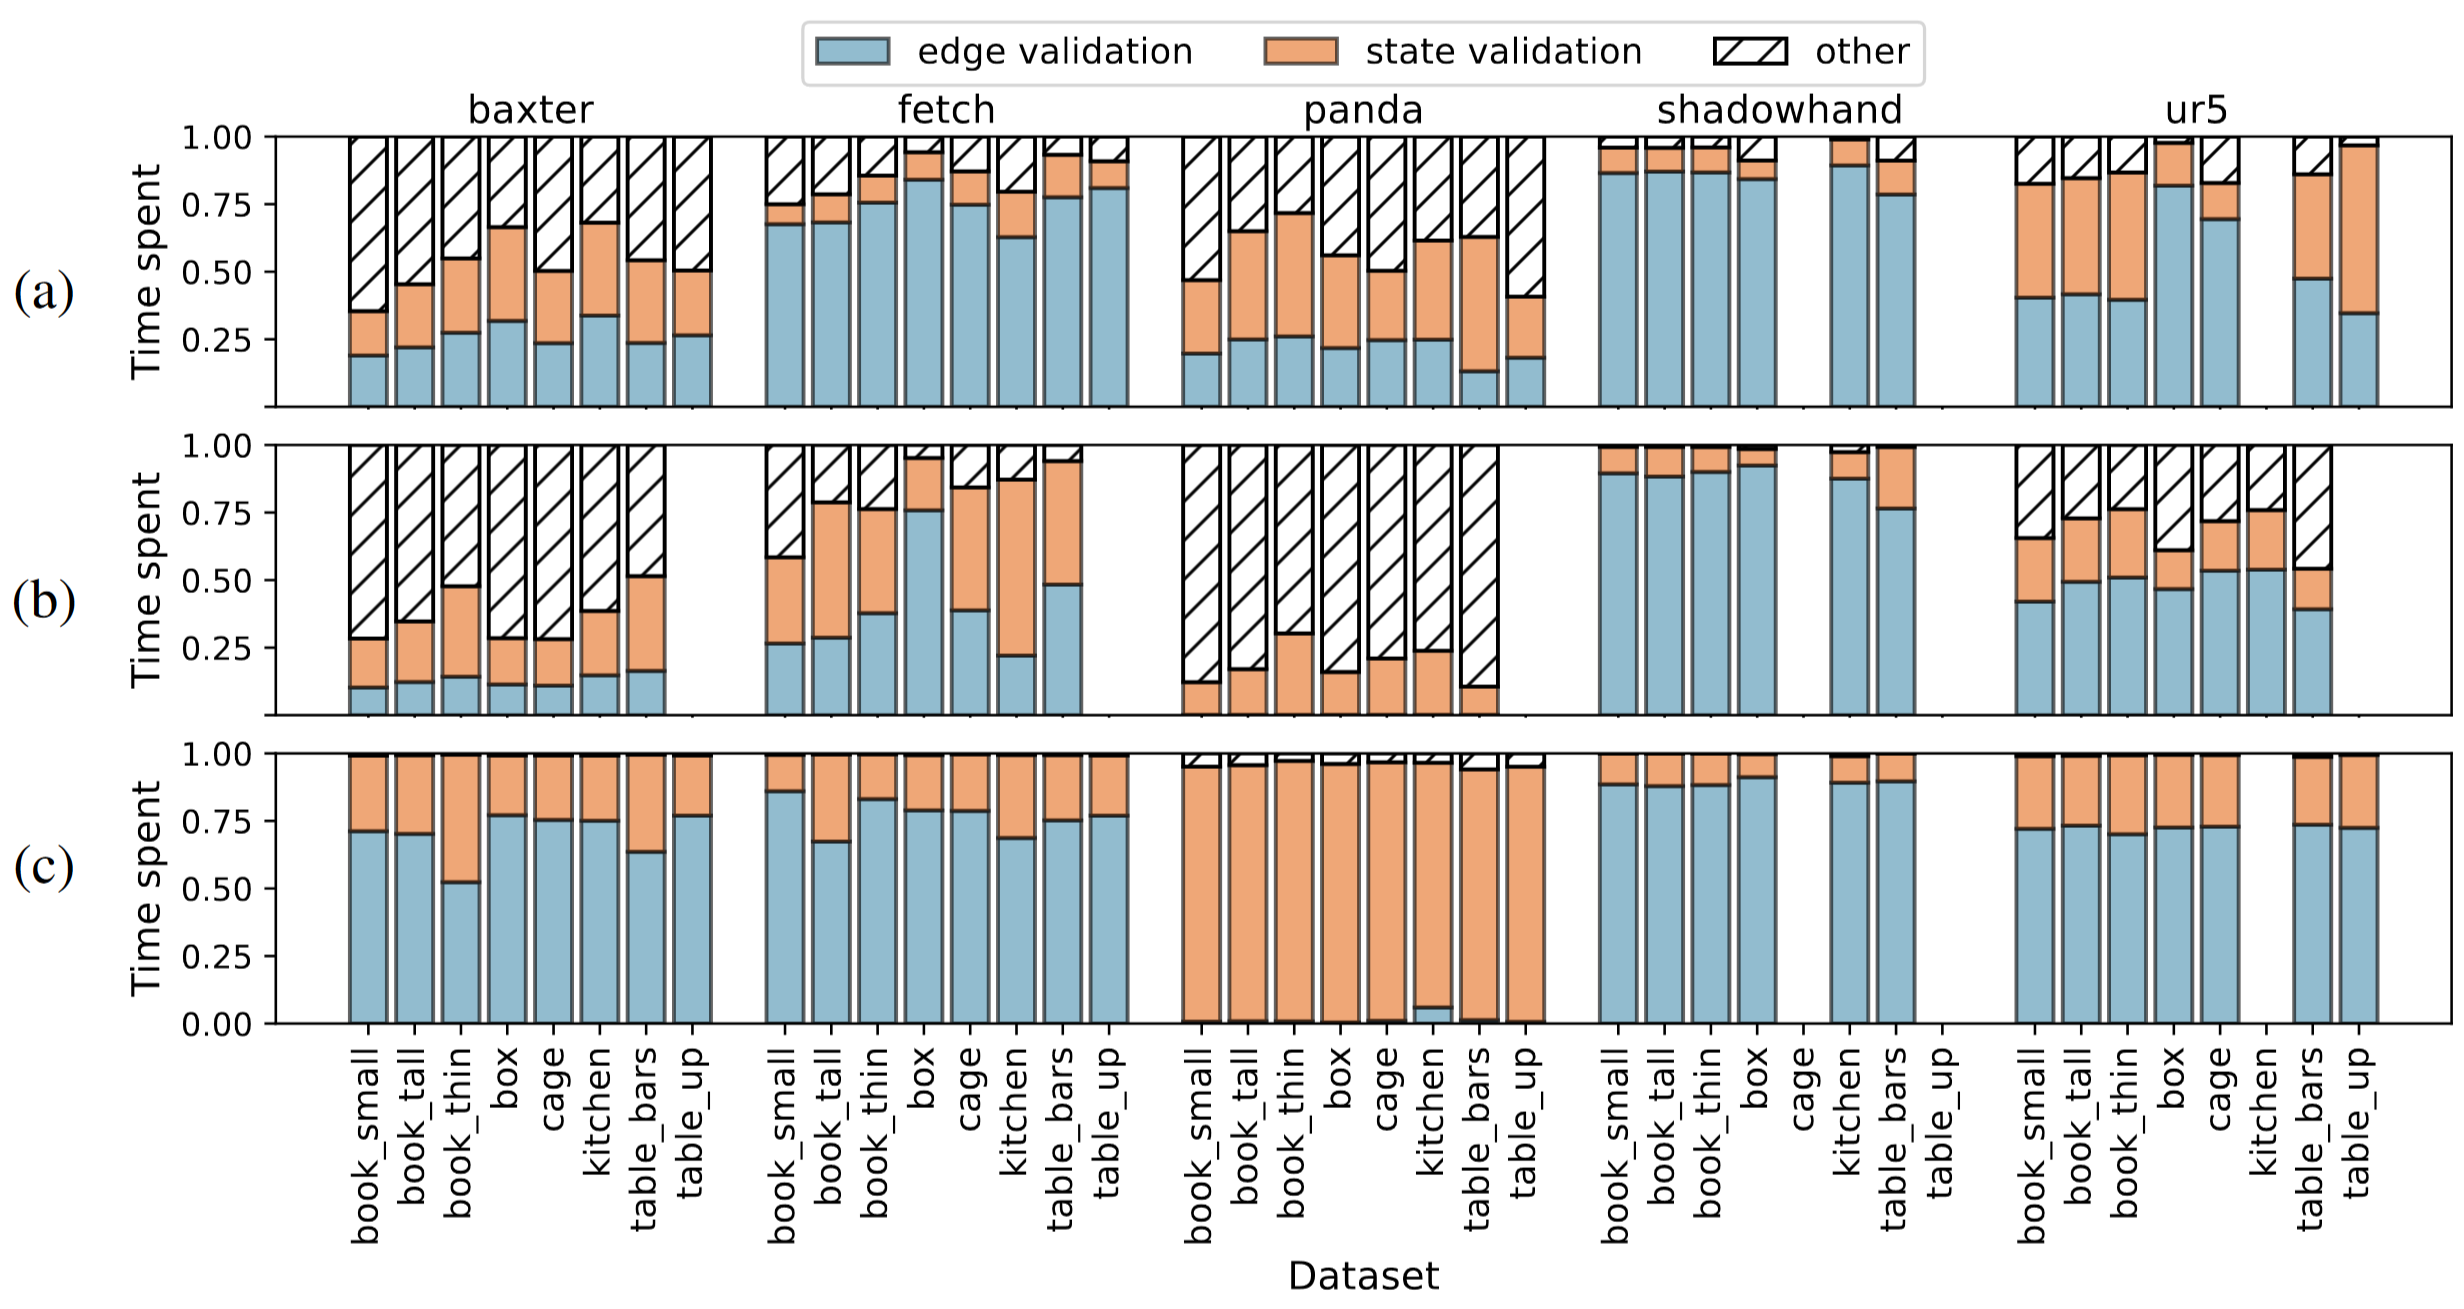
\includegraphics[width=\textwidth]{./assets/ev_sv_zoom.png}
\end{frame}

\begin{frame}{Scene Collisions vs Self Collisions}
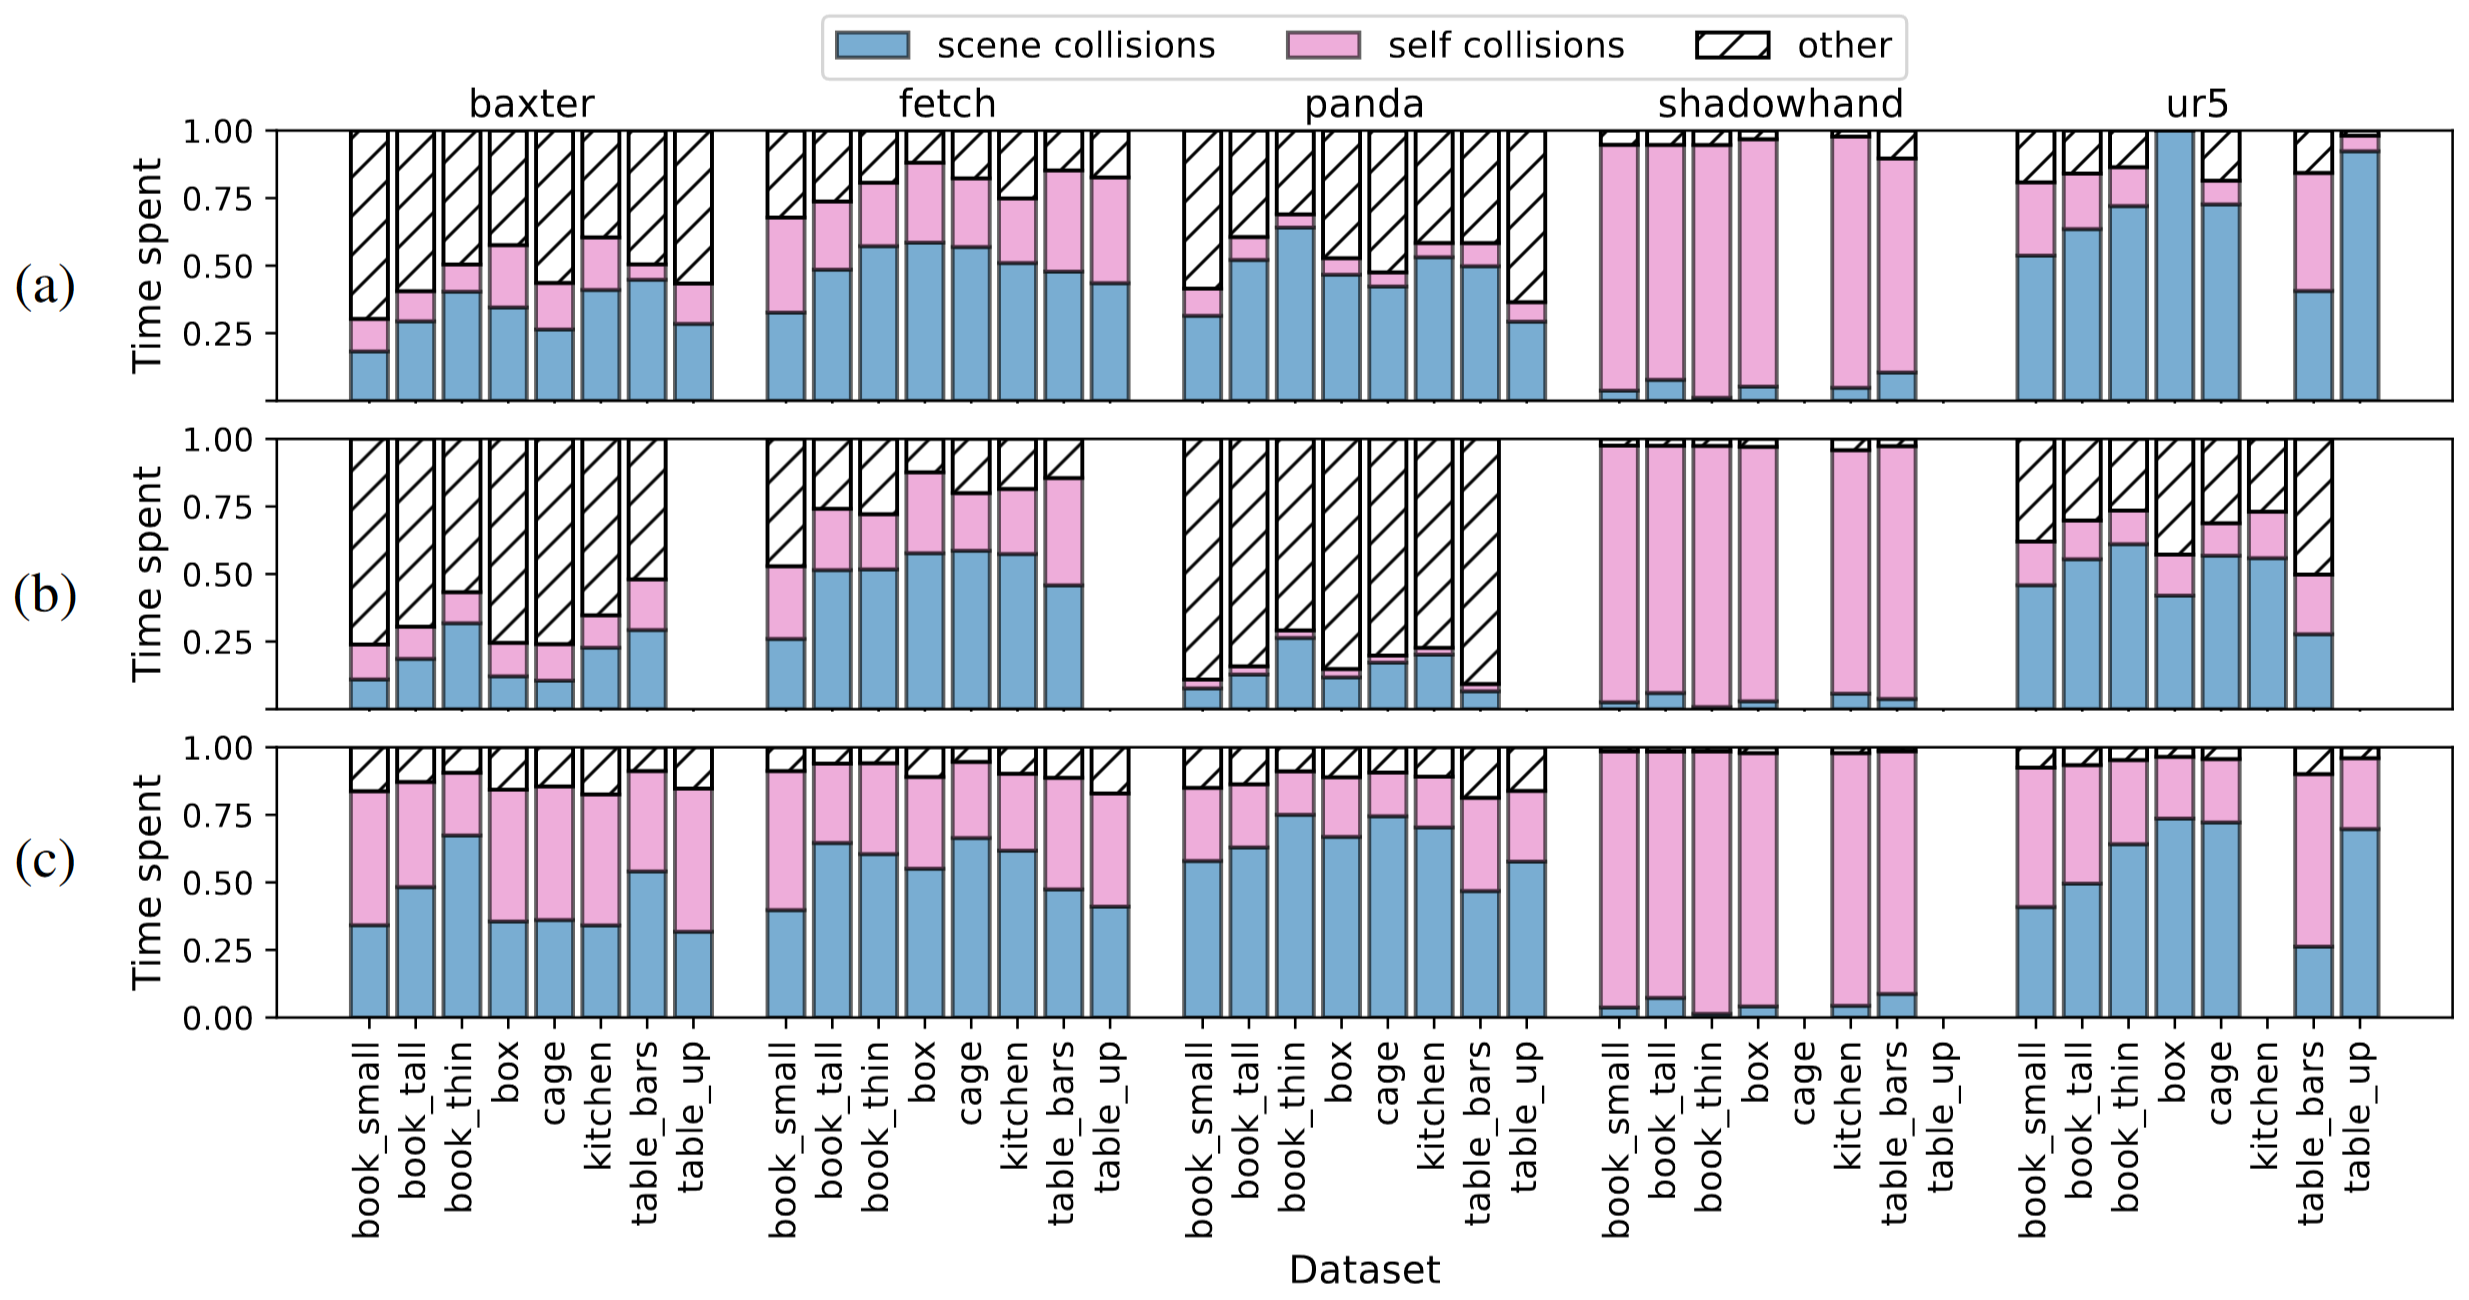
\includegraphics[width=\textwidth]{./assets/sc_sc_zoom.png}
\end{frame}

\section {TODO}

\begin{frame}{\todo{Things to improve}}
\begin{enumerate}
\item Buff Future Work Slide
\item Strengths \& Weaknesses both need a lift
\item explanation of raked mv. animate.
\item \textsc{fk} explanation on slide \ref{p_primitives} using featherstone ex 4.3 (ty radhika)
\item cite things better, add bibliography
\item Figures post-presentation
\end{enumerate}
\end{frame}
\end{document}